\begin{frame}
\end{frame}

\begin{frame}{Large-scale Pre-Training and Transfer}
\protect\hypertarget{large-scale-pre-training-and-transfer}{}
\begin{itemize}
\tightlist
\item
  Foundation models: transferable models pre-trained on large generic
  data

  \begin{itemize}
  \tightlist
  \item
    transfer across domains specific smaller datasets and tasks
  \item
    scaling laws: strong, efficient transfer - large models pre-trained
    on large data
  \end{itemize}
\end{itemize}

\center{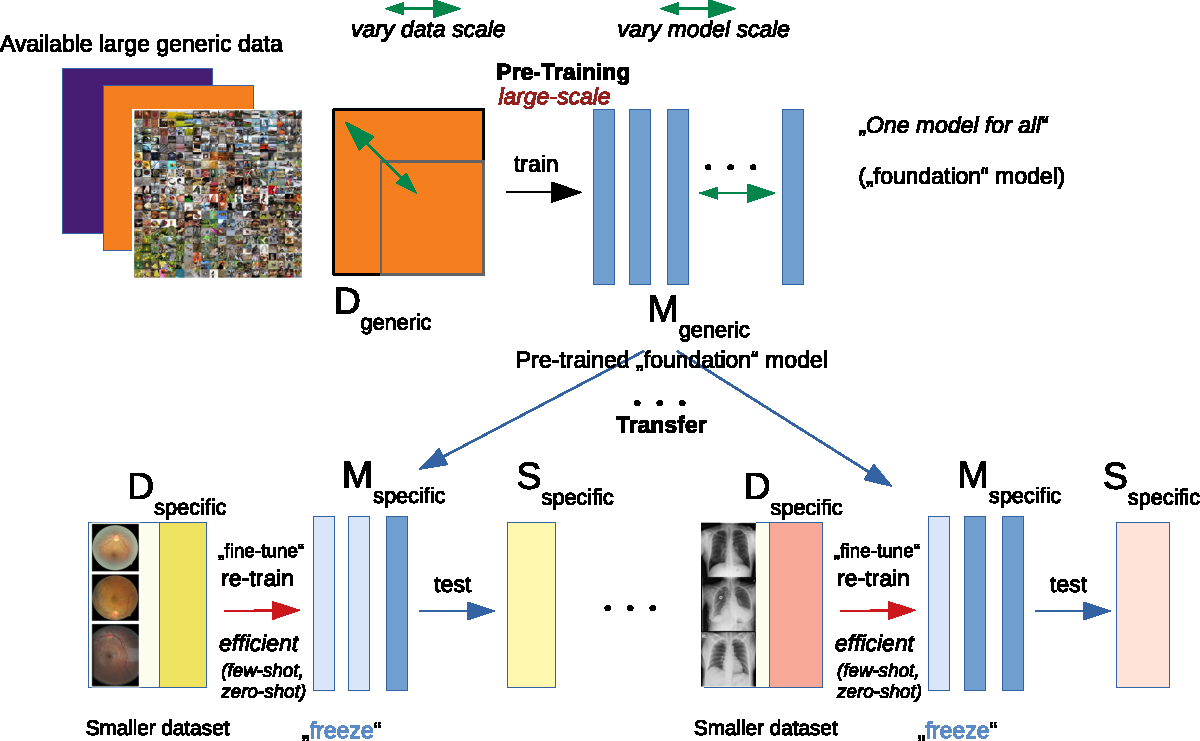
\includegraphics[width=0.8\textwidth]{../images/Pretrain_Transfer_Foundation_Model_mod.pdf}}
\end{frame}

\begin{frame}{Large-scale Pre-Training and Transfer}
\protect\hypertarget{large-scale-pre-training-and-transfer-1}{}
\begin{itemize}
\tightlist
\item
  Supervised learning on generic images : relating images to low
  information labels
\end{itemize}

\center{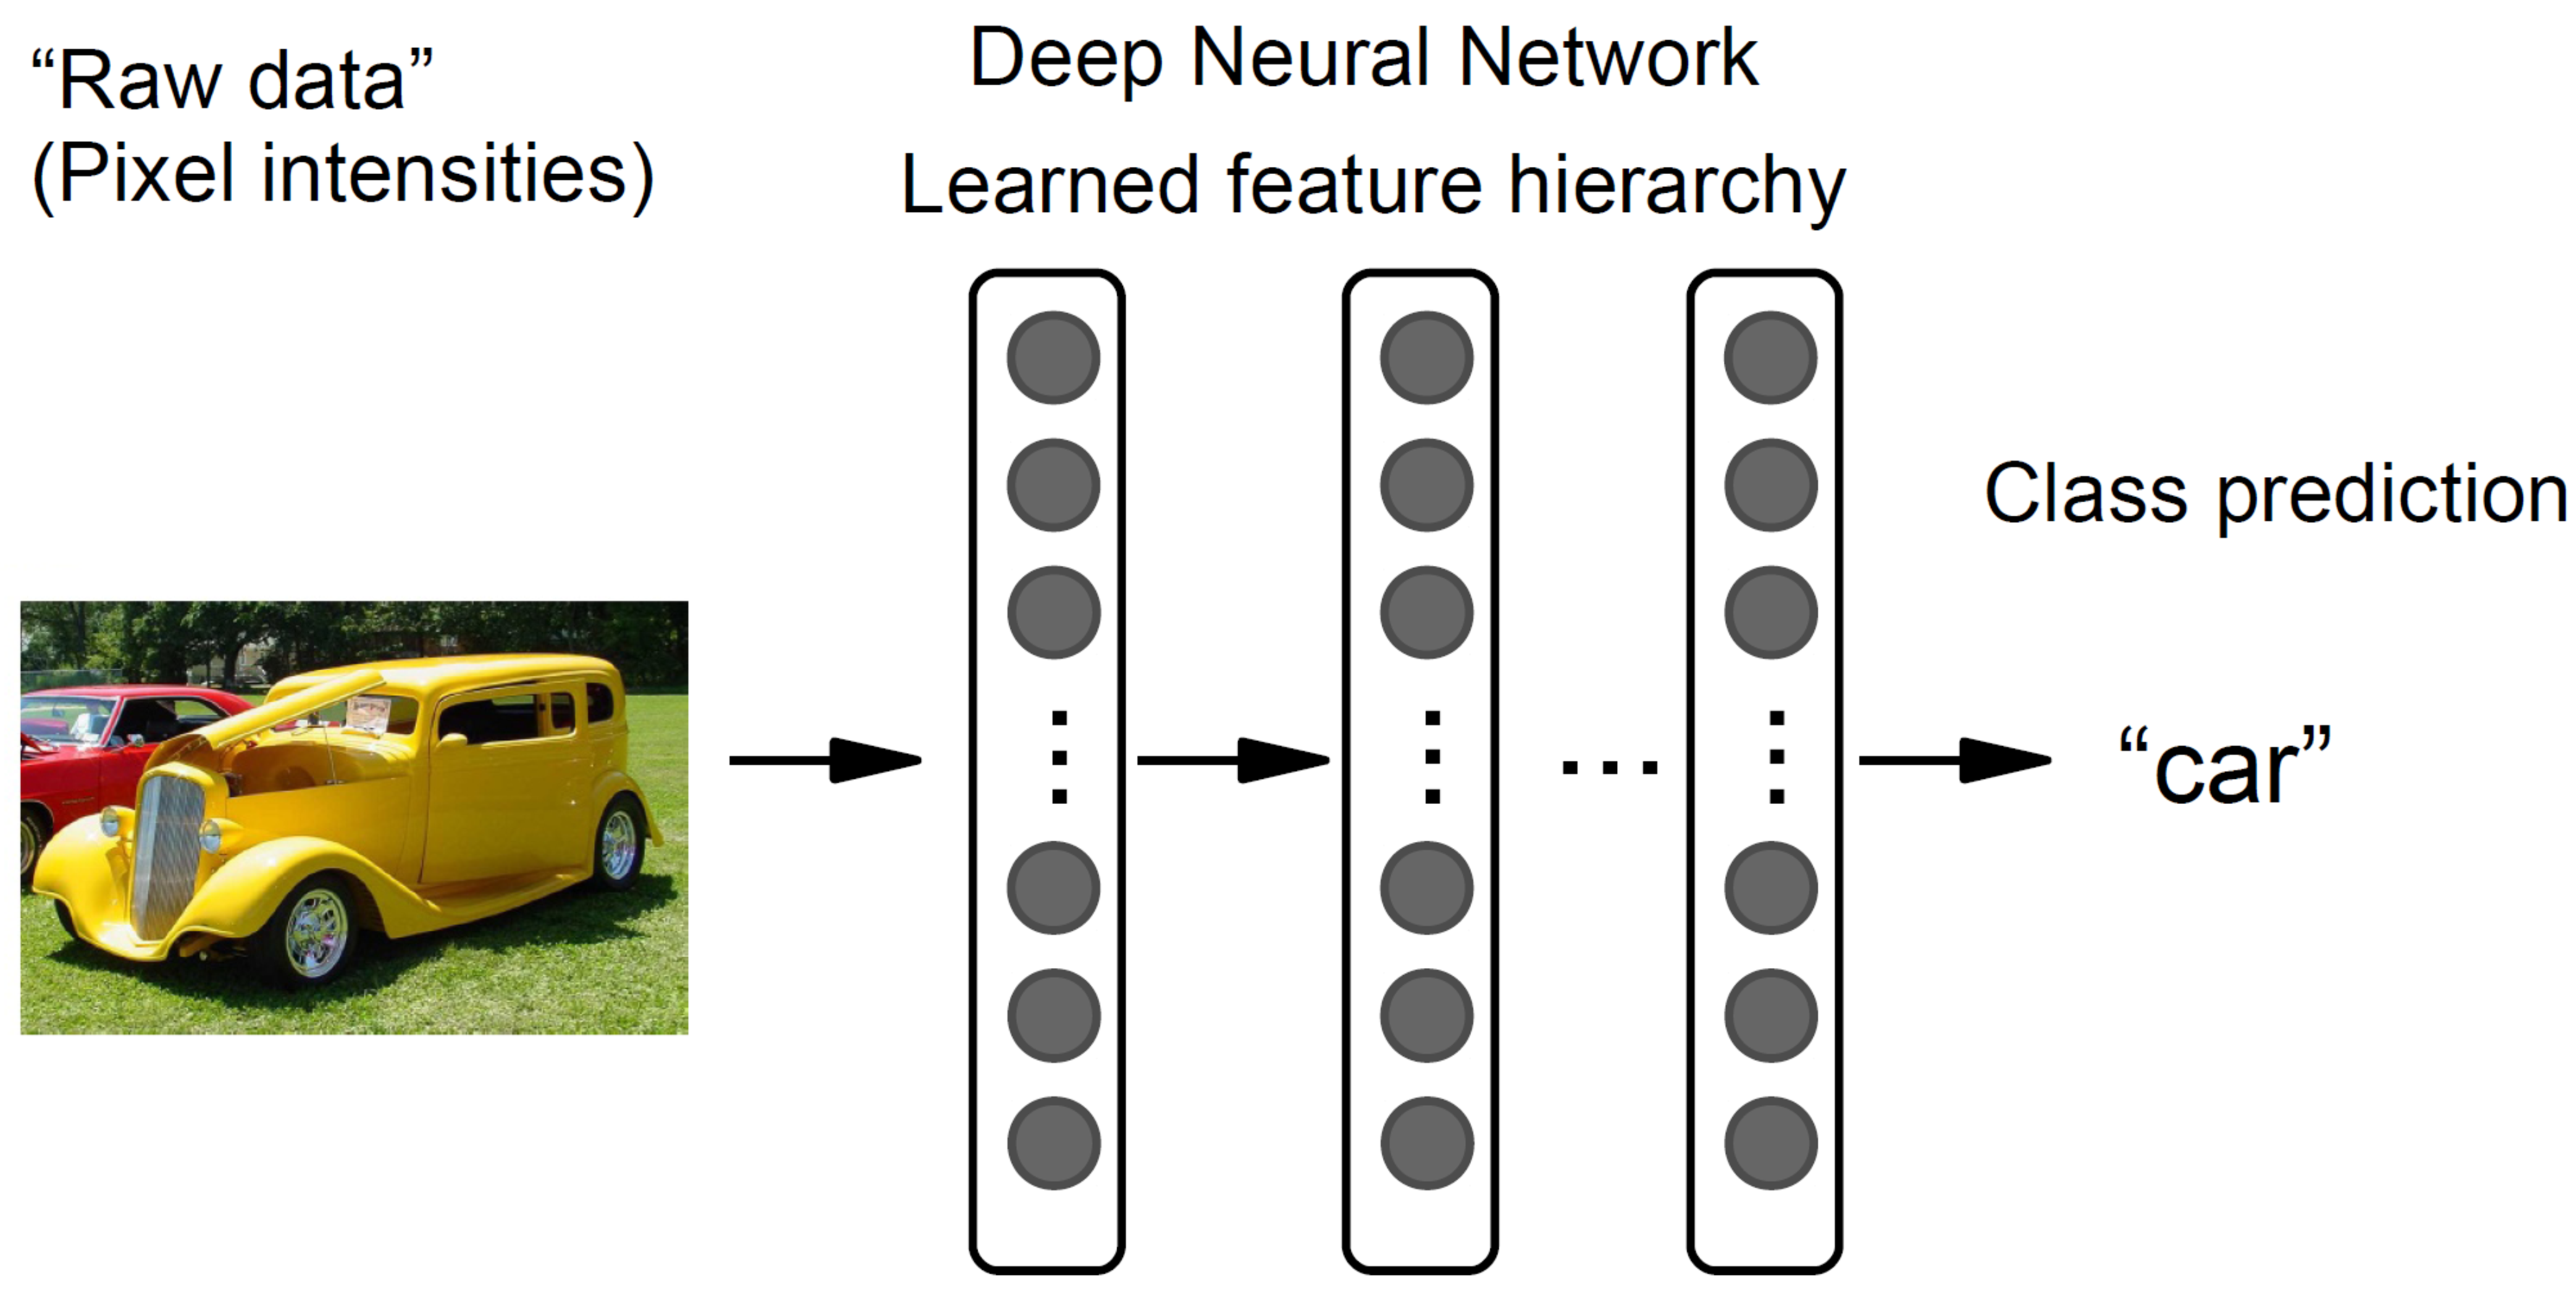
\includegraphics[width=0.8\textwidth]{../images/Supervised_Learning_Car_Image.pdf}}
\end{frame}

\begin{frame}{Large-scale Pre-Training and Transfer}
\protect\hypertarget{large-scale-pre-training-and-transfer-2}{}
\begin{itemize}
\tightlist
\item
  Supervised learning : relating high information input signal to low
  information labels

  \begin{itemize}
  \tightlist
  \item
    fixed, rather small label ``vocabulary''
  \end{itemize}
\end{itemize}

\center{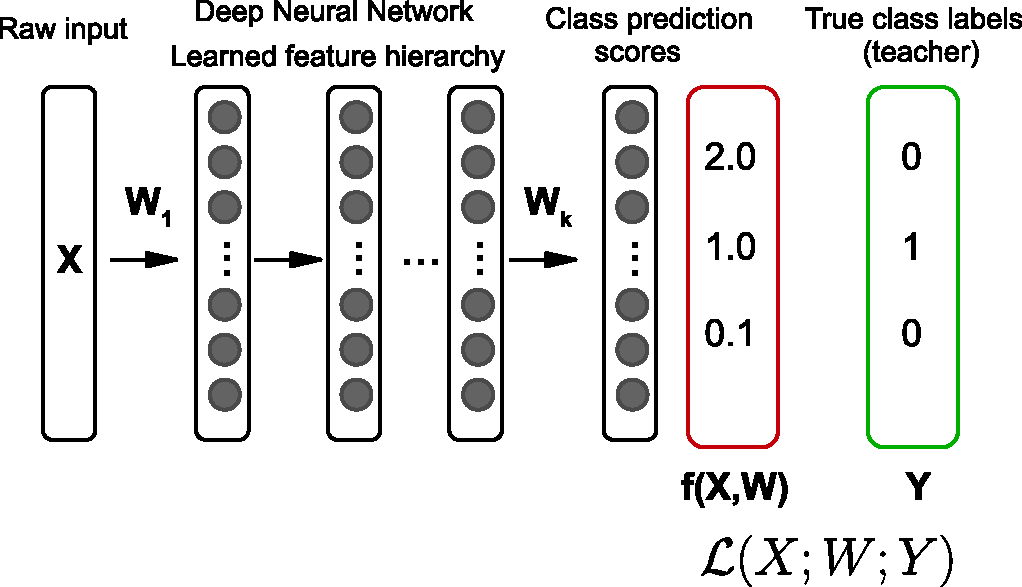
\includegraphics[width=0.8\textwidth]{../images/Supervised_Learning_Labels_Teacher_mod.pdf}}
\end{frame}

\begin{frame}{Large-scale Pre-Training and Transfer}
\protect\hypertarget{large-scale-pre-training-and-transfer-3}{}
\begin{itemize}
\tightlist
\item
  Scaling Laws: Larger Data, Larger Models - better transfer
\item
  Supervised learning on ImageNet-1k : pre-trained models transferable

  \begin{itemize}
  \tightlist
  \item
    pre-train on ImageNet-1k - transfer across various downstream tasks
  \end{itemize}
\item
  Problem: Human-labeled data poorly scalable

  \begin{itemize}
  \tightlist
  \item
    \textbf{ImageNet-21k}: \textbf{14x} larger
  \item
    \textbf{JFT-300M}: \textbf{300x} larger - pseudo-labels
  \end{itemize}
\end{itemize}

\center{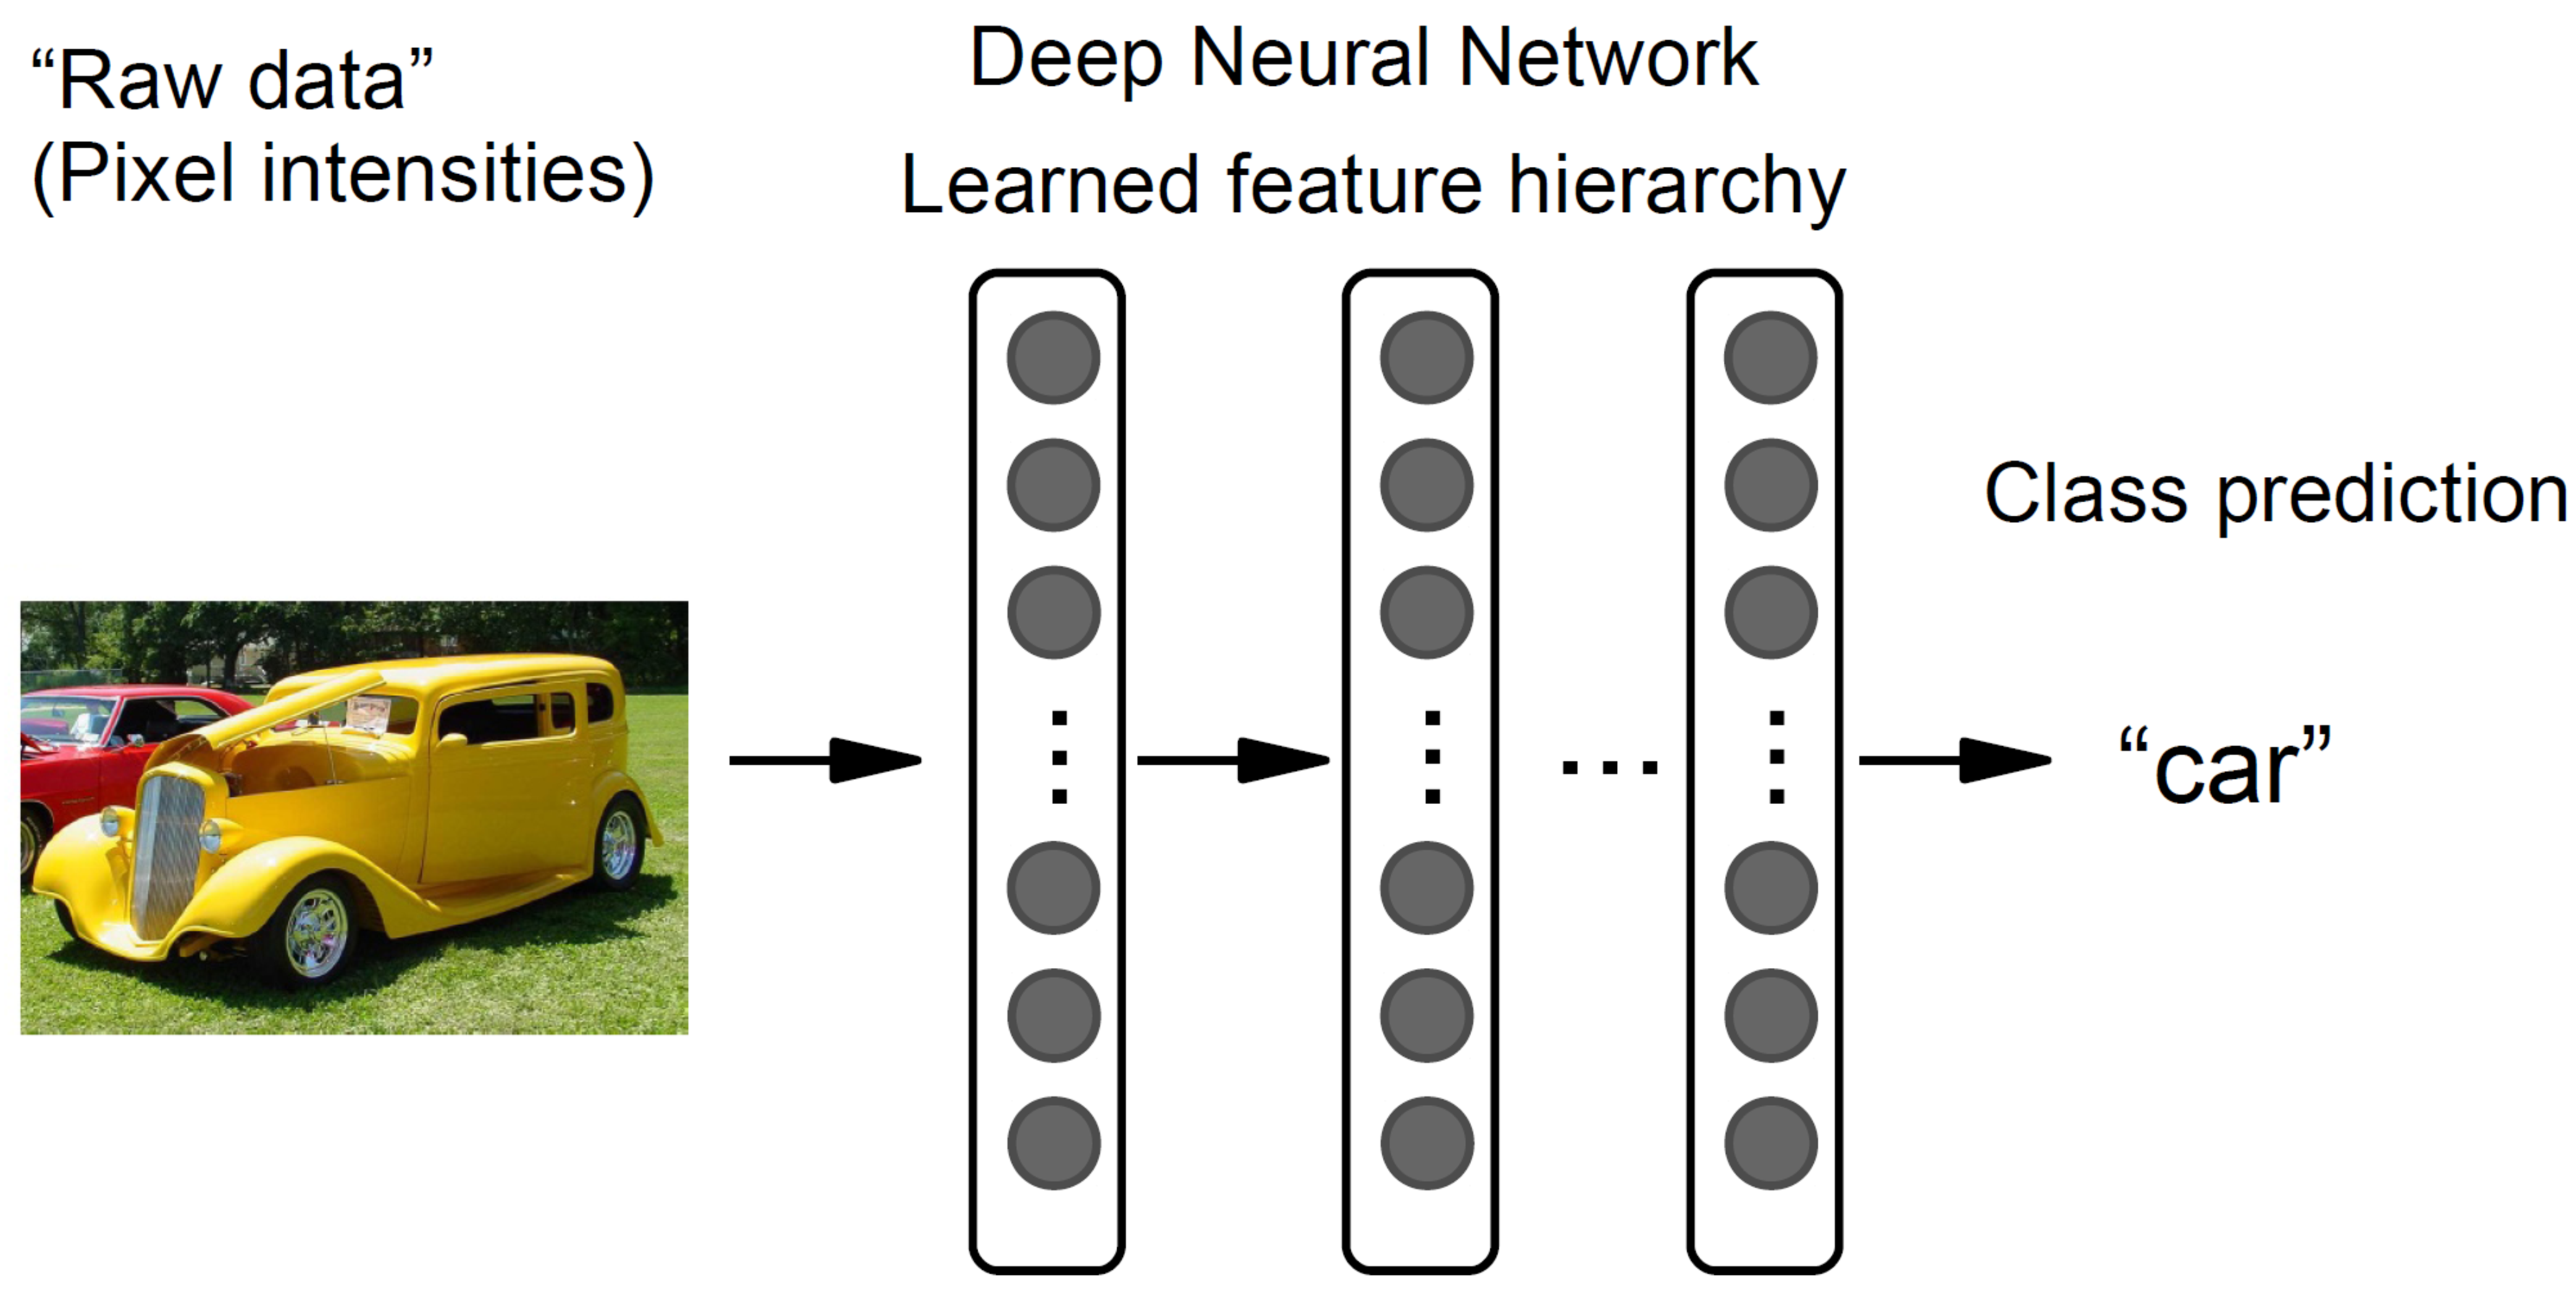
\includegraphics[width=0.6\textwidth]{../images/Supervised_Learning_Car_Image.pdf}}
\end{frame}

\begin{frame}{Large-scale Pre-Training and Transfer}
\protect\hypertarget{large-scale-pre-training-and-transfer-4}{}
\begin{itemize}
\tightlist
\item
  Scaling Laws: Larger Data, Larger Models - better transfer
\item
  Supervised learning on ImageNet-1k : pre-trained models transferable

  \begin{itemize}
  \tightlist
  \item
    pre-train on ImageNet-1k - transfer across various downstream tasks
  \end{itemize}
\item
  Problem: poor zero-shot transfer, poor robustness to data distribution
  shift

  \begin{itemize}
  \tightlist
  \item
    \textbf{ImageNet-21k}: \textbf{14x} larger
  \item
    \textbf{JFT-300M}: \textbf{300x} larger - pseudo-labels
  \end{itemize}
\end{itemize}

\center{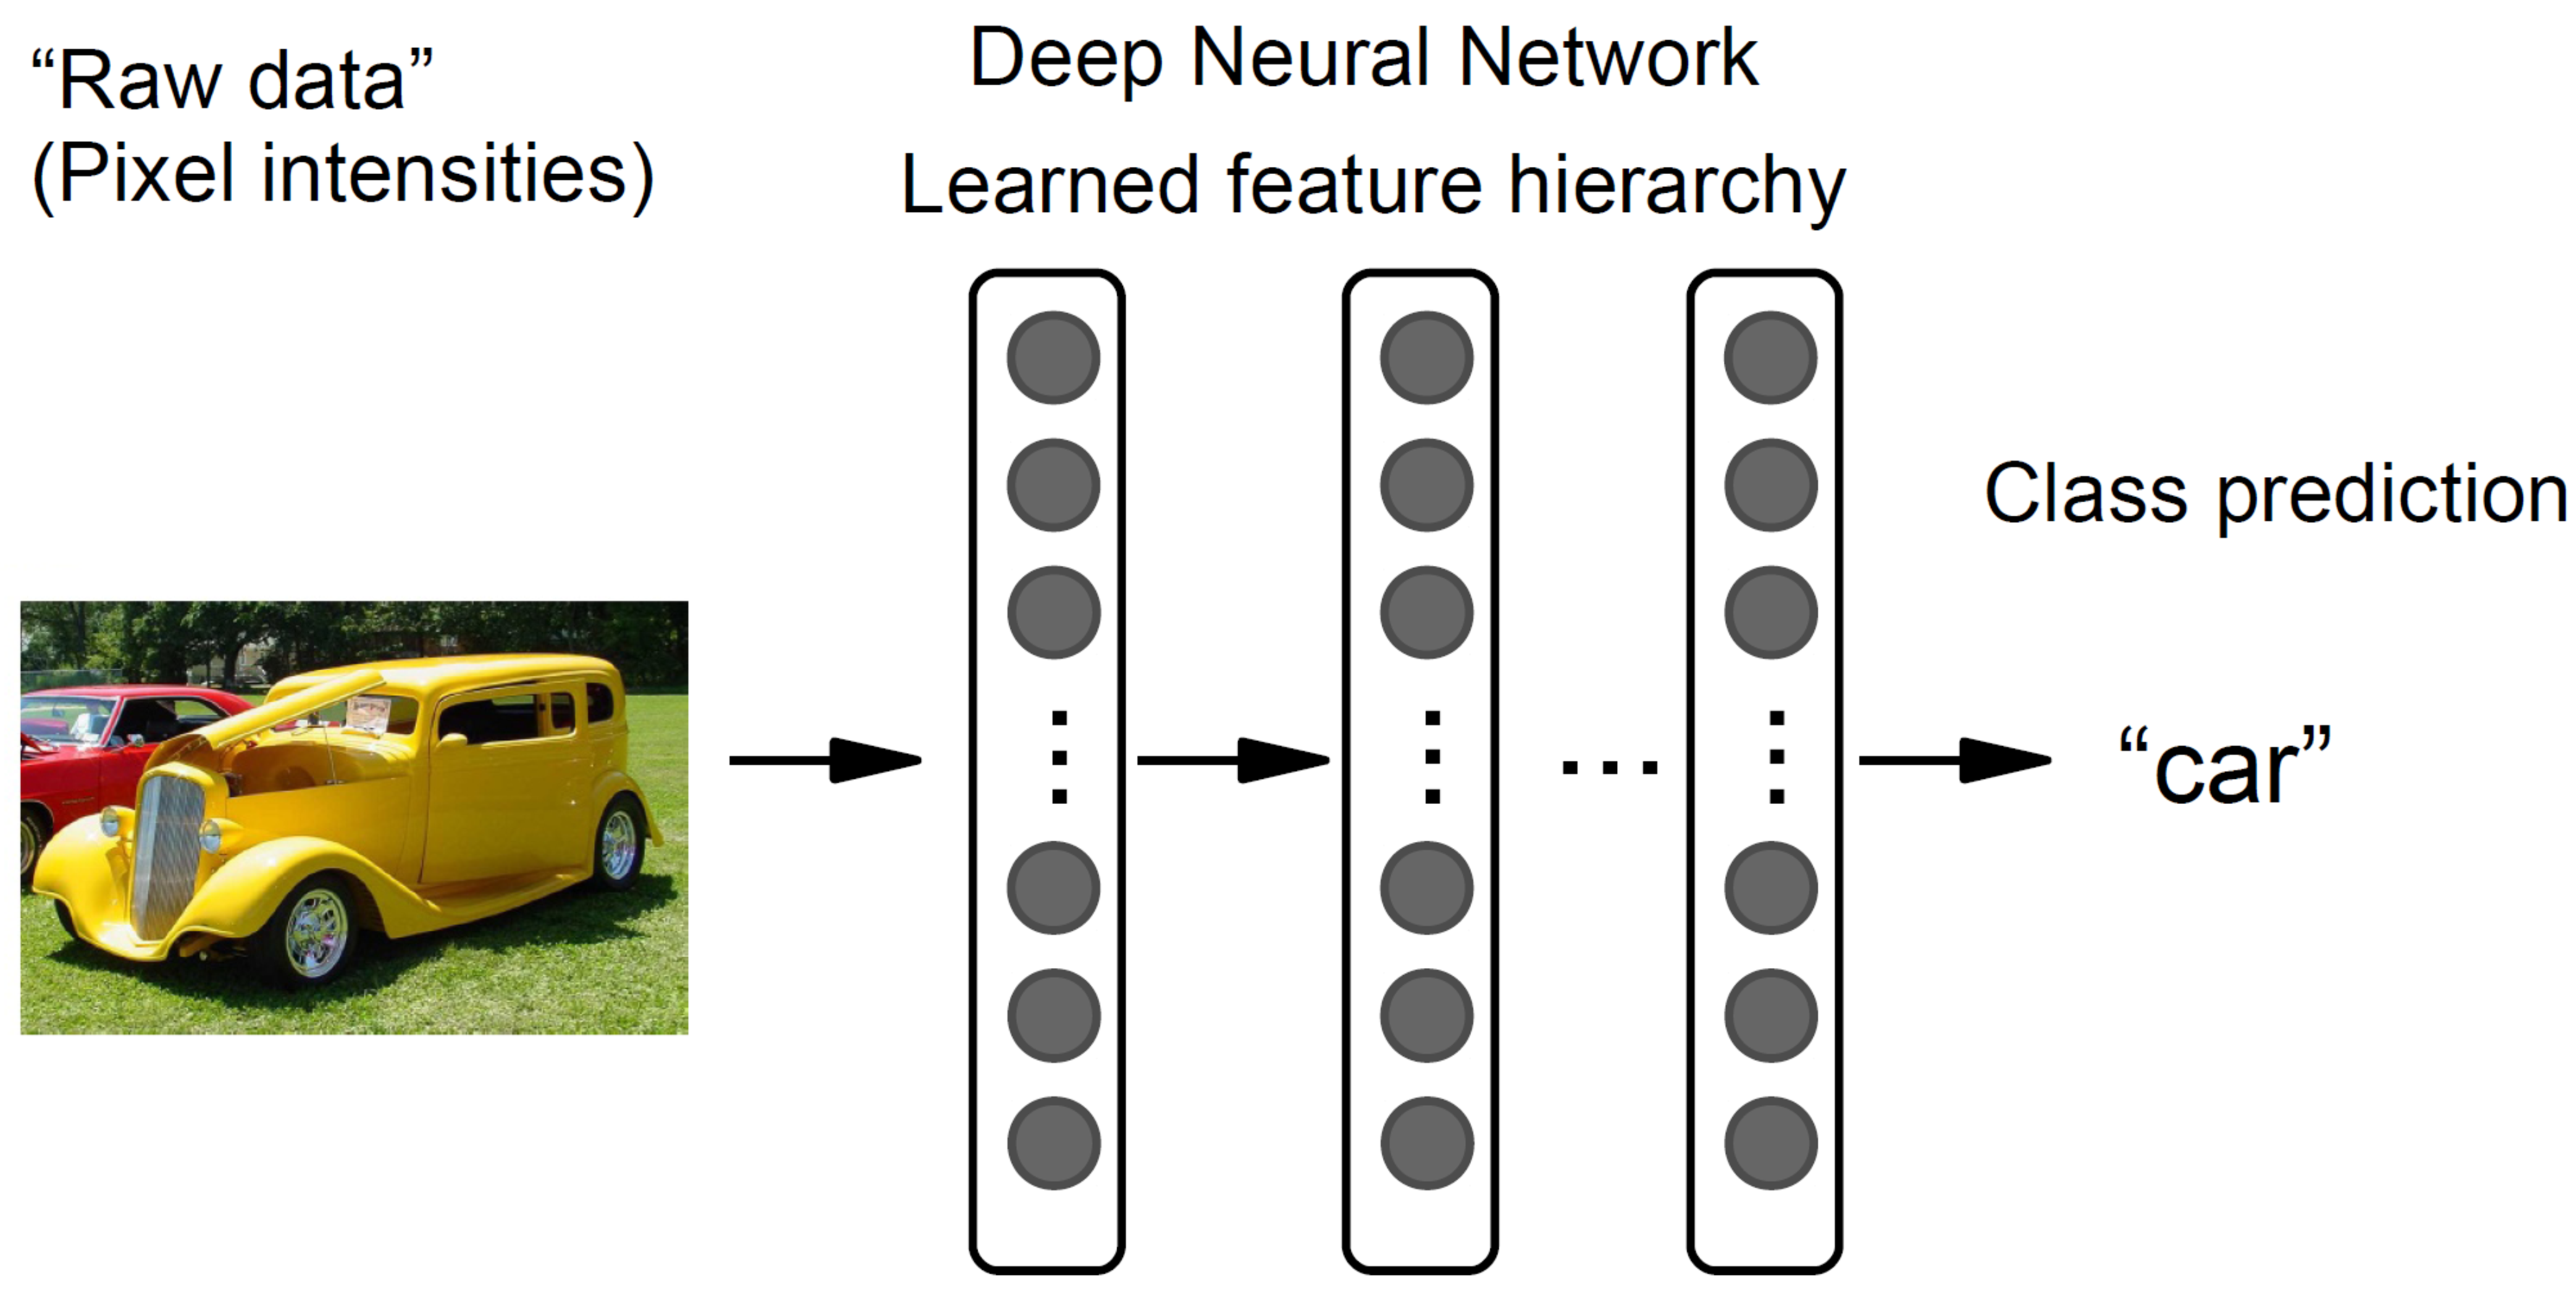
\includegraphics[width=0.6\textwidth]{../images/Supervised_Learning_Car_Image.pdf}}
\end{frame}

\begin{frame}{Large-scale Pre-Training and Transfer}
\protect\hypertarget{large-scale-pre-training-and-transfer-5}{}
\begin{itemize}
\tightlist
\item
  Scaling Laws: Larger Data, Larger Models - better transfer
\item
  Supervised learning on ImageNet-1k : pre-trained models transferable

  \begin{itemize}
  \tightlist
  \item
    pre-train on ImageNet-1k - transfer across various downstream tasks
  \end{itemize}
\item
  Problem: poor zero-shot transfer, poor robustness to data distribution
  shift

  \begin{itemize}
  \tightlist
  \item
    \textbf{ImageNet-21k}: \textbf{14x} larger
  \item
    \textbf{JFT-300M}: \textbf{300x} larger - pseudo-labels
  \end{itemize}
\end{itemize}

\center{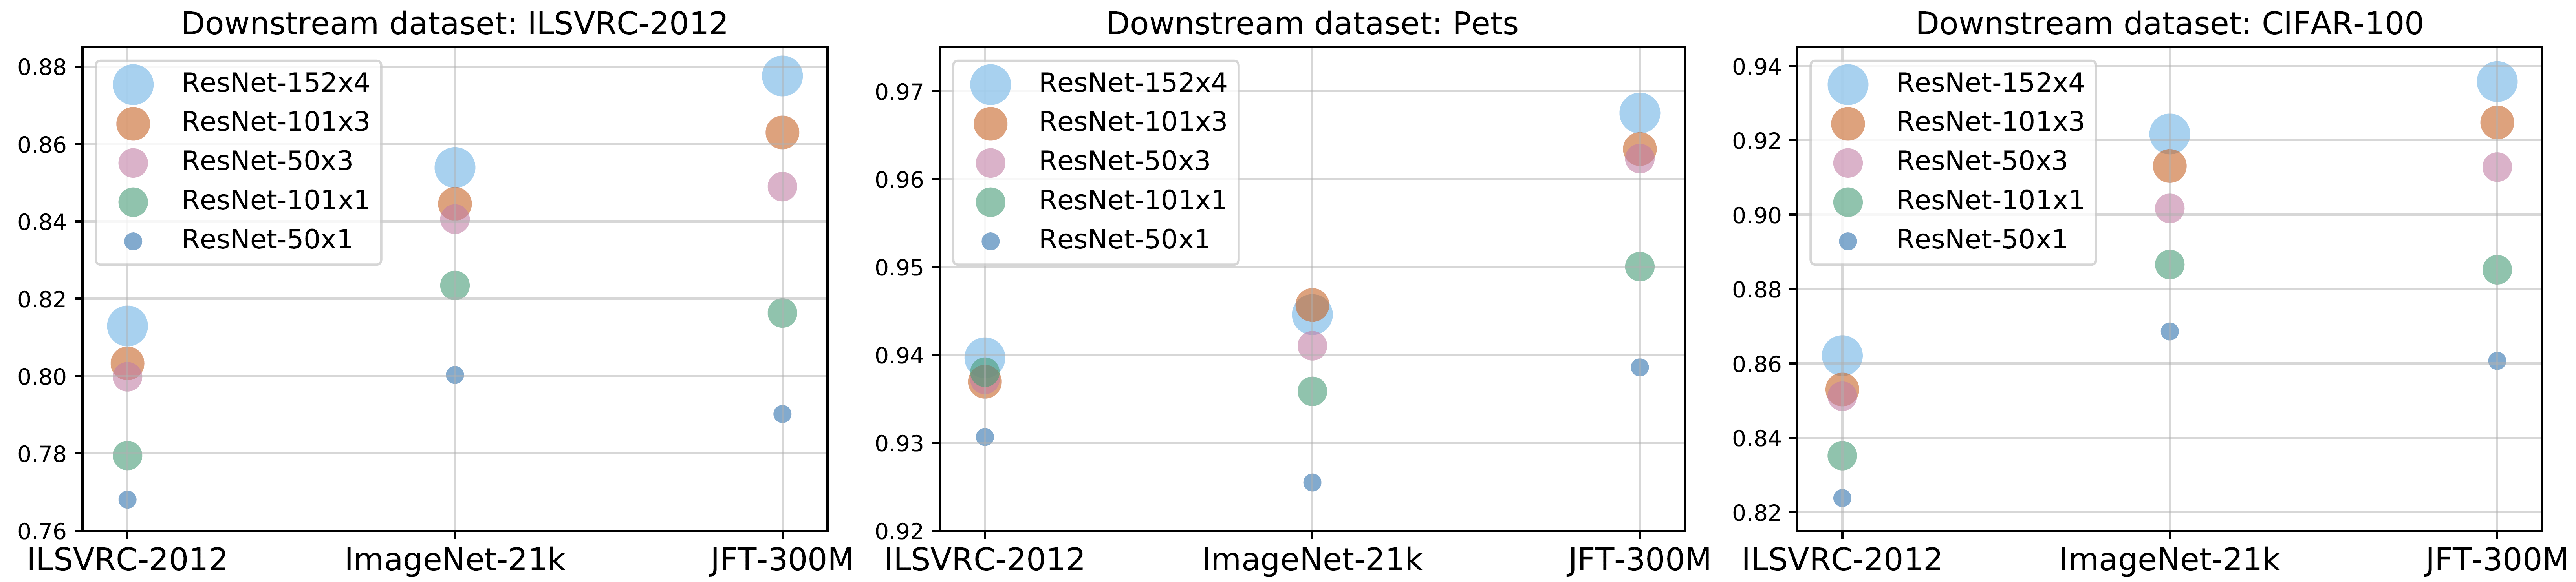
\includegraphics[width=\textwidth]{../images/Pretraining_BiT_Data_Networks_smaller_larger.png}}

\footnote<.->{\tiny BiT - Big Transfer, Kolesnikov et al, ECCV, 2020}
\end{frame}

\begin{frame}{Large-scale Pre-Training and Transfer}
\protect\hypertarget{large-scale-pre-training-and-transfer-6}{}
\begin{itemize}
\tightlist
\item
  Scalable data: unlabeled or pseudo-labeled data
\item
  \textbf{Unsupervised}, \textbf{Self-Supervised} learning in different
  flavors

  \begin{itemize}
  \tightlist
  \item
    human-made labels not required
  \end{itemize}
\item
  Often, using auxiliary tasks - self-supervised learning

  \begin{itemize}
  \tightlist
  \item
    contrastive losses (SimCLR, DINO), reconstruction based losses (eg
    VAEs, MAE, Diffusion models), \ldots{}
  \item
    adversarial losses (eg. GANs -\textgreater{} see Day 5 Special!)
  \end{itemize}
\end{itemize}

\center{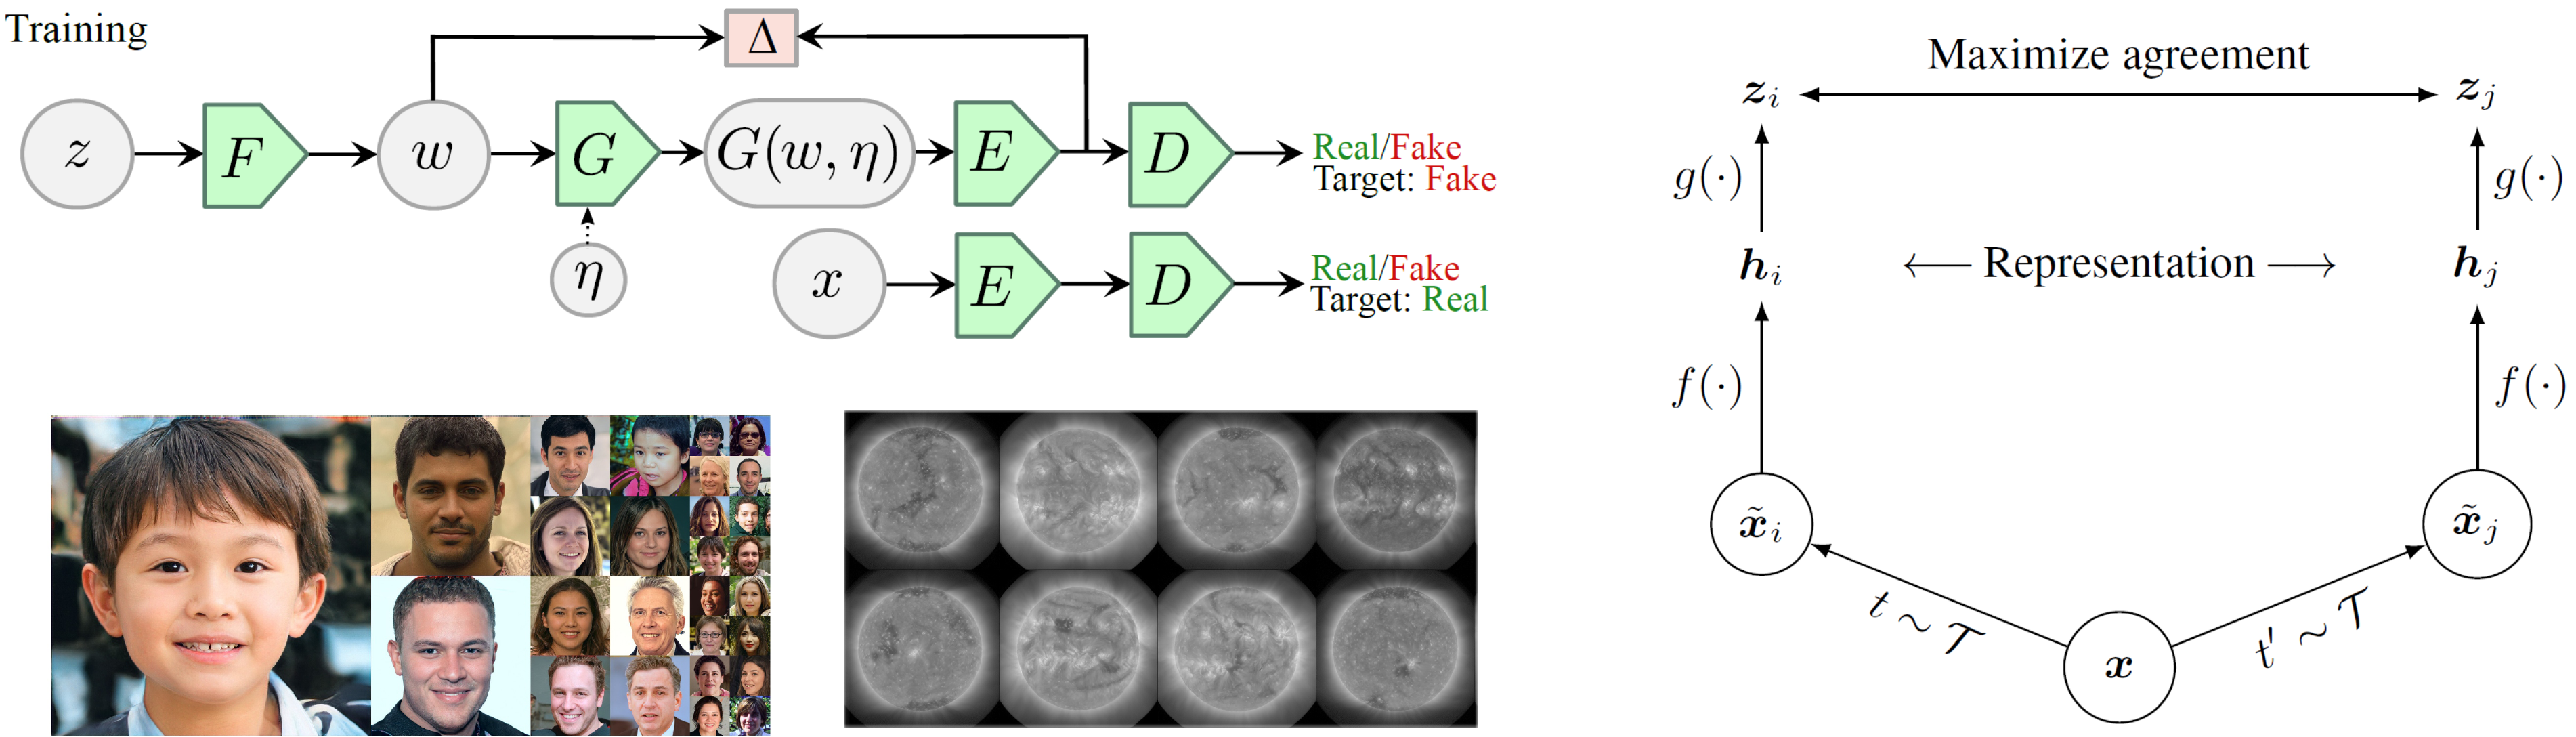
\includegraphics[width=\textwidth]{../images/unsupervised_learning_overview.png}}

\footnote<.->{\tiny Pidhorskyi et al, 2020; Effenberger et al, 2020;
  Chen et al, 2020}
\end{frame}

\begin{frame}{Large-scale Pre-Training and Transfer}
\protect\hypertarget{large-scale-pre-training-and-transfer-7}{}
\begin{itemize}
\tightlist
\item
  Scalable data: unlabeled data
\item
  Contrastive losses: construct losses from transformed pairs of inputs
\end{itemize}

\begin{columns}[T]
\begin{column}{0.5\textwidth}
\small

\[
\mathbf{z}_i = g(\mathbf{h}_i),\quad
\mathbf{z}_j = g(\mathbf{h}_j),\quad
\text{sim}(\mathbf{z}_i, \mathbf{z}_j) = \frac{\mathbf{z}_i^\top\mathbf{z}_j}{\|\mathbf{z}_i\| \|\mathbf{z}_j\|}
\]

\vspace*{-0.2cm}

\[
\mathcal{L}_{i,j} = - \log\frac{\exp(\text{sim}(\mathbf{z}_i, \mathbf{z}_j) / \tau)}{\sum_{k=1}^{2n} \mathbf{1}_{[k \neq i]} \exp(\text{sim}(\mathbf{z}_i, \mathbf{z}_k) / \tau)}
\]

\normalsize

\center{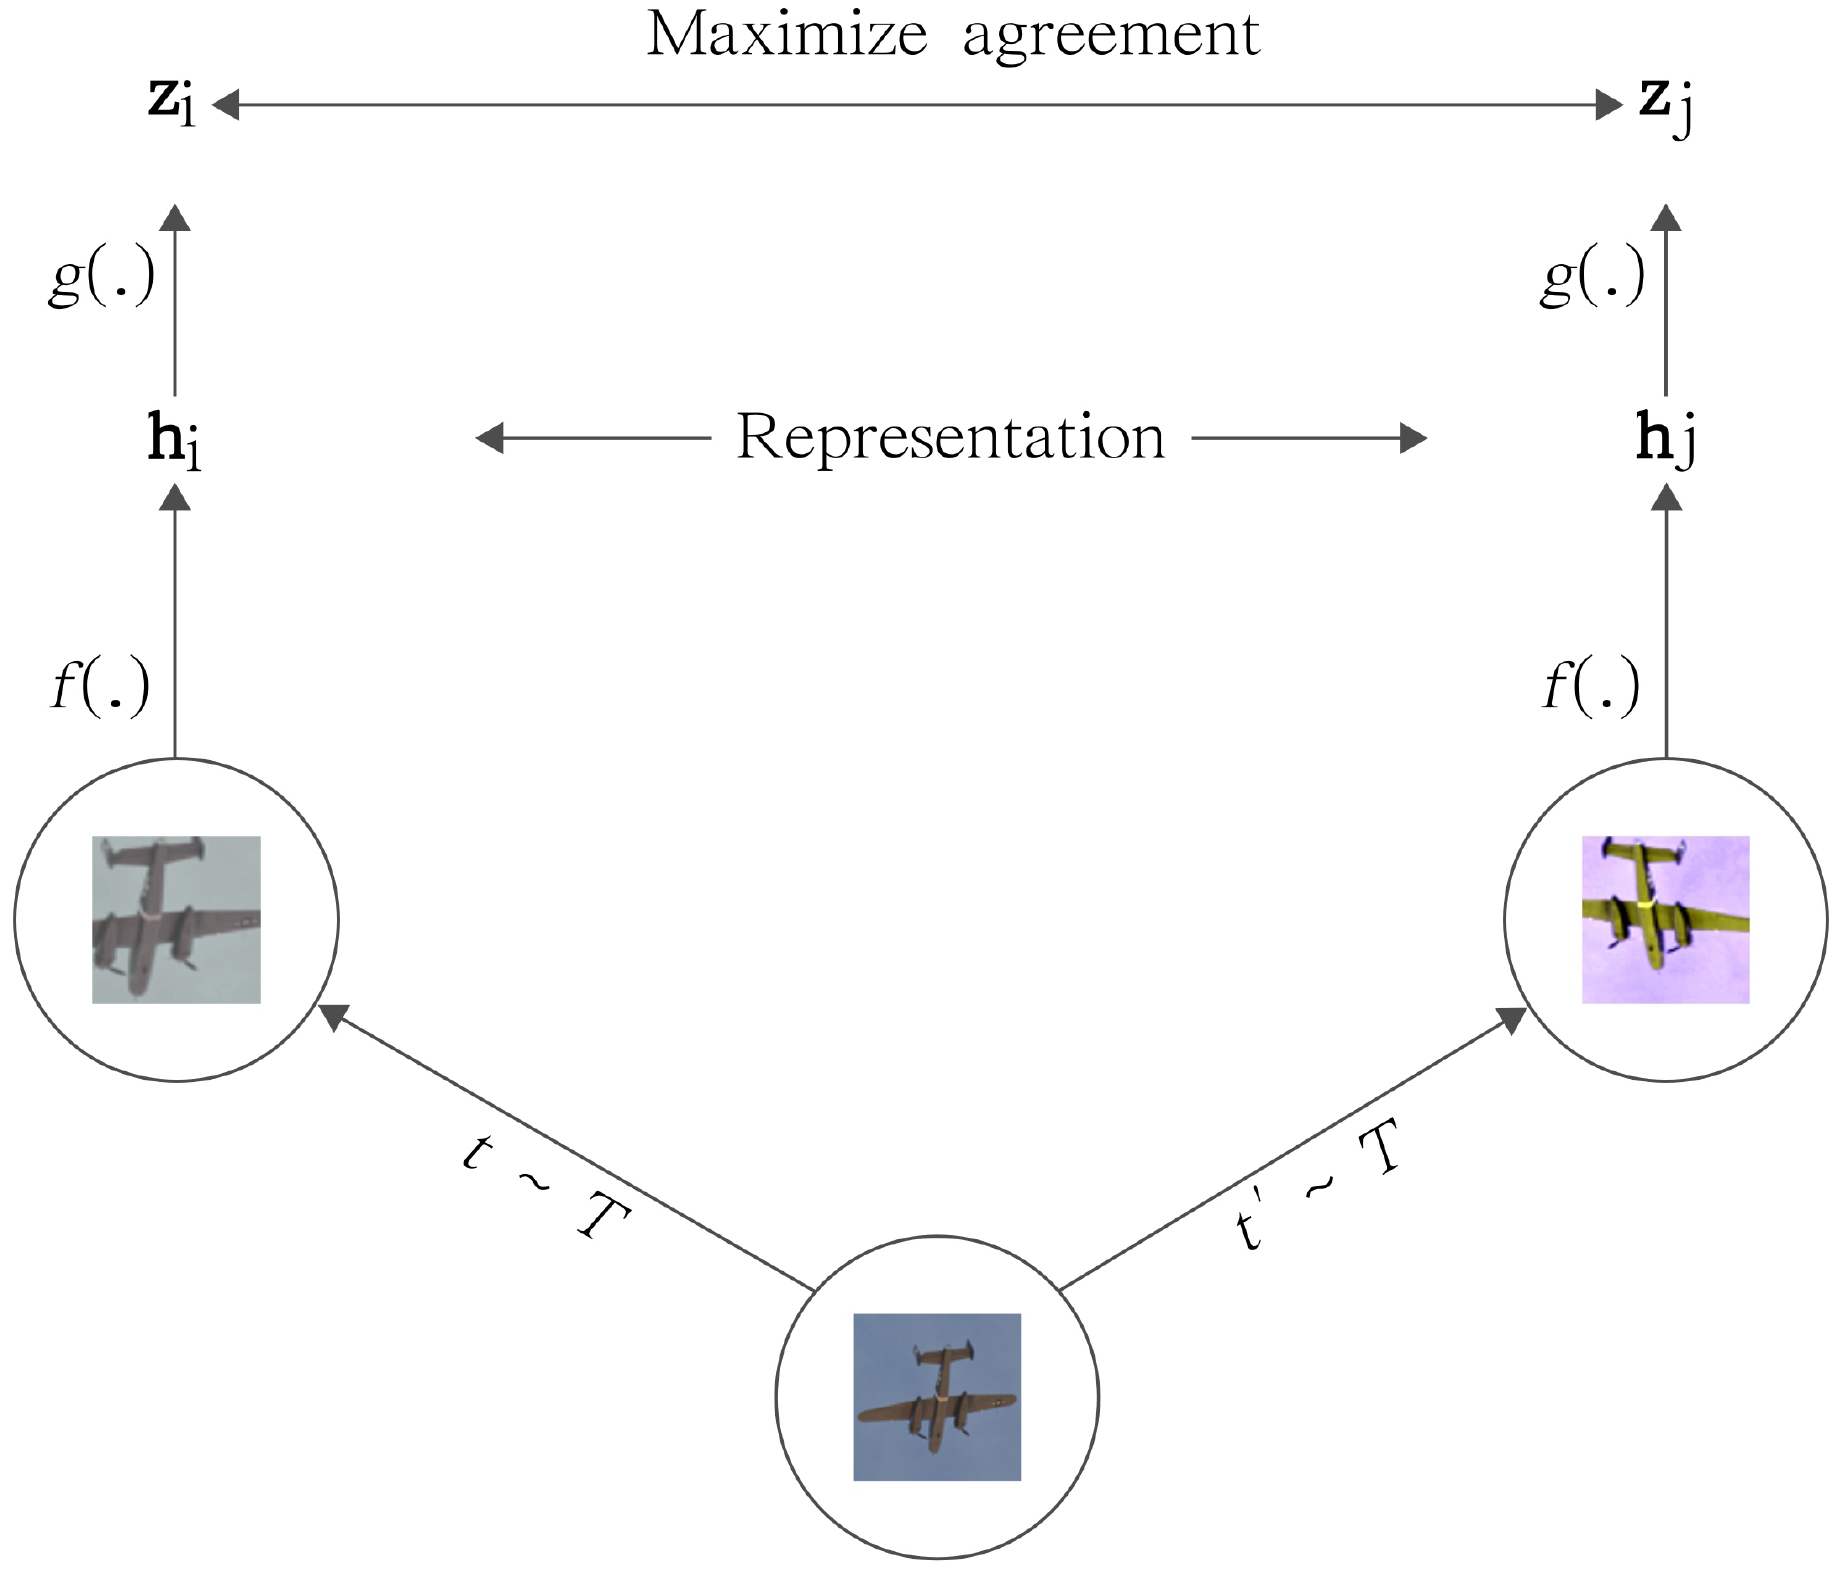
\includegraphics[width=0.7\textwidth]{../images/SimCLR_plane.png}}
\end{column}

\begin{column}{0.5\textwidth}
\center{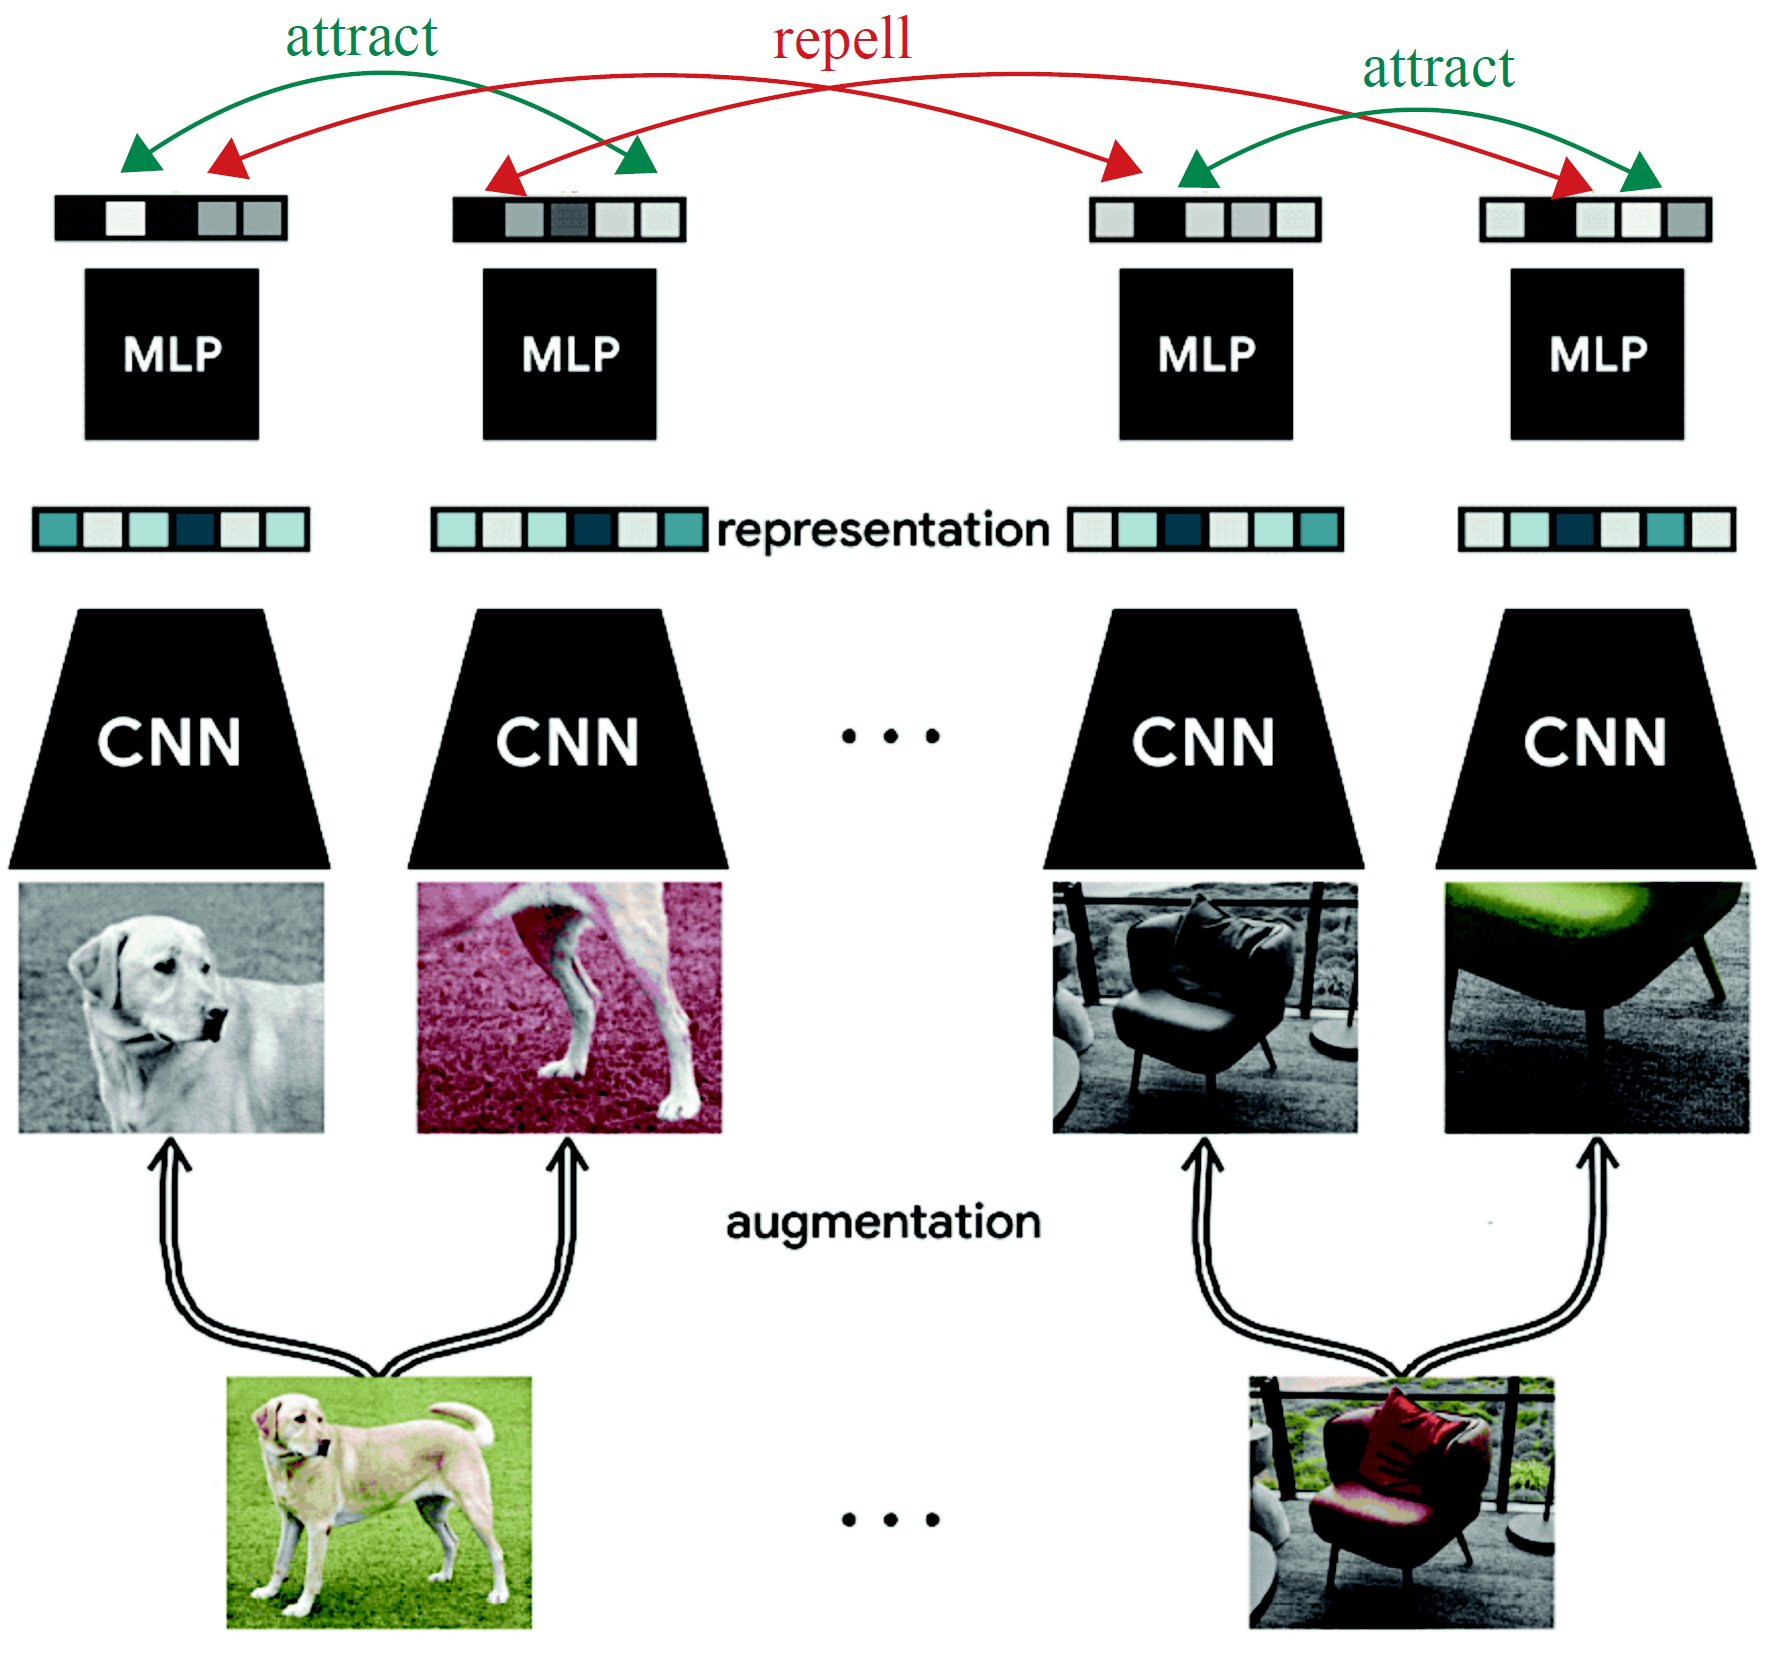
\includegraphics[width=0.7\textwidth]{../images/SimCLR_Attract_Repell.png}}
\end{column}
\end{columns}

\footnote<.->{\tiny Chen et al, 2020}
\end{frame}

\begin{frame}{Large-scale Pre-Training and Transfer}
\protect\hypertarget{large-scale-pre-training-and-transfer-8}{}
\begin{itemize}
\tightlist
\item
  Scalable data: unlabeled data
\item
  Contrastive losses: larger models - better self-supervised learning
\item
  Evidence for better representations in larger networks after
  self-supervised pre-training
\end{itemize}

\center{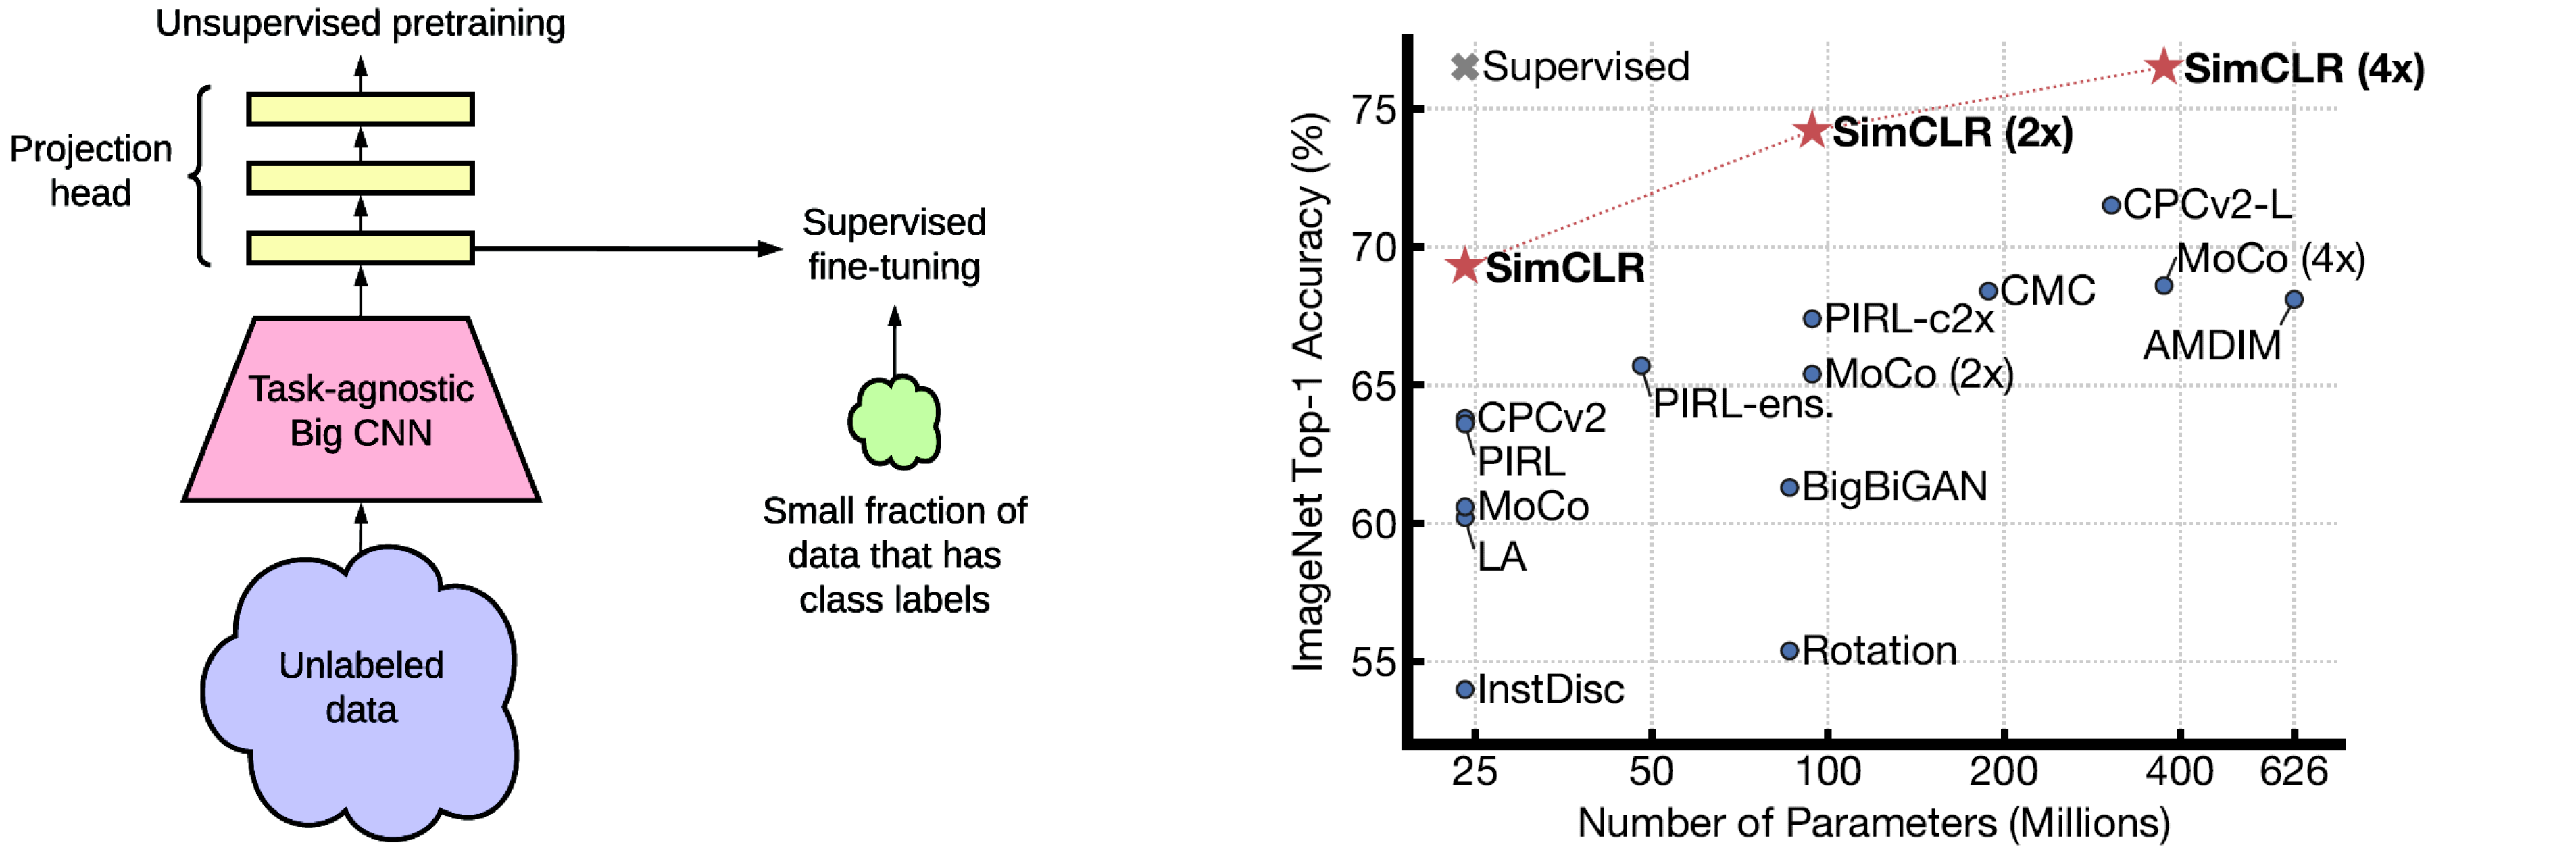
\includegraphics[width=0.8\textwidth]{../images/SimCLR_Linear_Classifier_Slide.png}}

\footnote<.->{\tiny Chen et al, 2020}
\end{frame}

\begin{frame}{Large-scale Pre-Training and Transfer}
\protect\hypertarget{large-scale-pre-training-and-transfer-9}{}
\begin{itemize}
\tightlist
\item
  Scalable data: weakly aligned image-text pairs from public Internet
\item
  CLIP: foundation language-vision model for large-scale representation
  learning

  \begin{itemize}
  \tightlist
  \item
    \textbf{self-supervised, open vocabulary pre-training on image-text
    pairs}
  \item
    very strong zero- and few-shot transfer across various downstream
    tasks
  \item
    strong robustness to data distribution shift
  \end{itemize}
\end{itemize}

\center{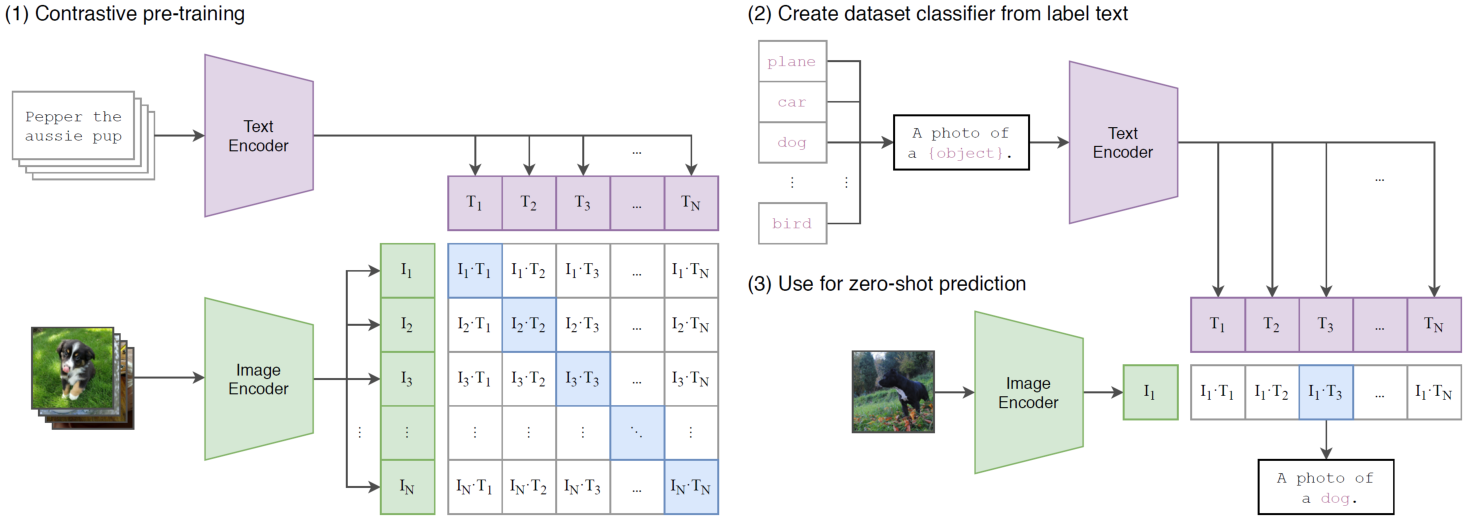
\includegraphics[width=0.85\textwidth]{../images/CLIP_Self_Supervised_Learning_mod.pdf}}

\footnote<.->{\tiny Radford, ICML, 2021}
\end{frame}

\begin{frame}{Large-scale Pre-Training and Transfer}
\protect\hypertarget{large-scale-pre-training-and-transfer-10}{}
\begin{itemize}
\tightlist
\item
  Scalable data: weakly aligned image-text pairs from public Internet
\item
  CLIP: foundation language-vision model for large-scale representation
  learning

  \begin{itemize}
  \tightlist
  \item
    self-supervised, open vocabulary pre-training on image-text pairs
  \item
    \textbf{very strong zero- and few-shot transfer across various
    downstream tasks}
  \item
    strong robustness to data distribution shift
  \end{itemize}
\end{itemize}

\center{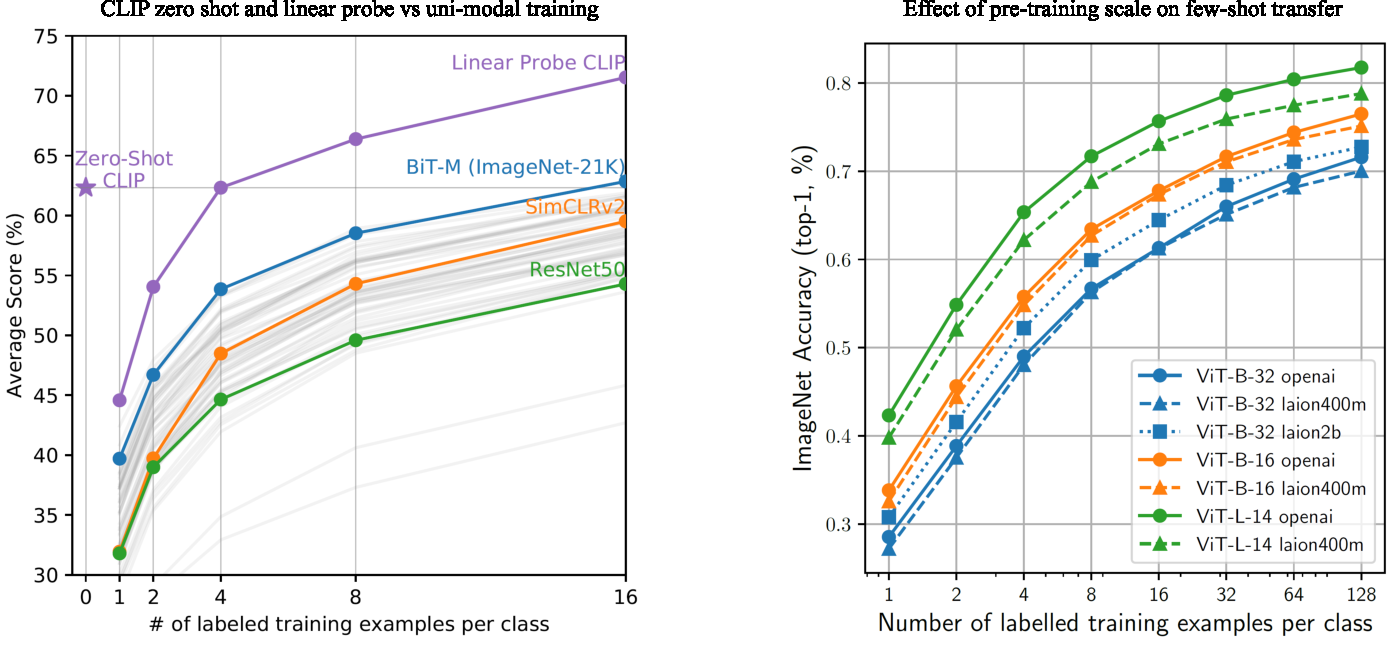
\includegraphics[width=0.8\textwidth]{../images/CLIP_Zero_Shot_Few_Shot_Scaling_mod.pdf}}

\footnote<.->{\tiny Radford, ICML, 2021; Schumann et al, NeurIPS 2022}
\end{frame}

\begin{frame}{Large-scale Pre-Training and Transfer}
\protect\hypertarget{large-scale-pre-training-and-transfer-11}{}
\begin{itemize}
\tightlist
\item
  Scalable data: weakly aligned image-text pairs from public Internet
\item
  CLIP: foundation language-vision model for large-scale representation
  learning

  \begin{itemize}
  \tightlist
  \item
    self-supervised, open vocabulary pre-training on image-text pairs
  \item
    very strong zero- and few-shot transfer across various downstream
    tasks
  \item
    \textbf{strong robustness to data distribution shift}
  \end{itemize}
\end{itemize}

\center{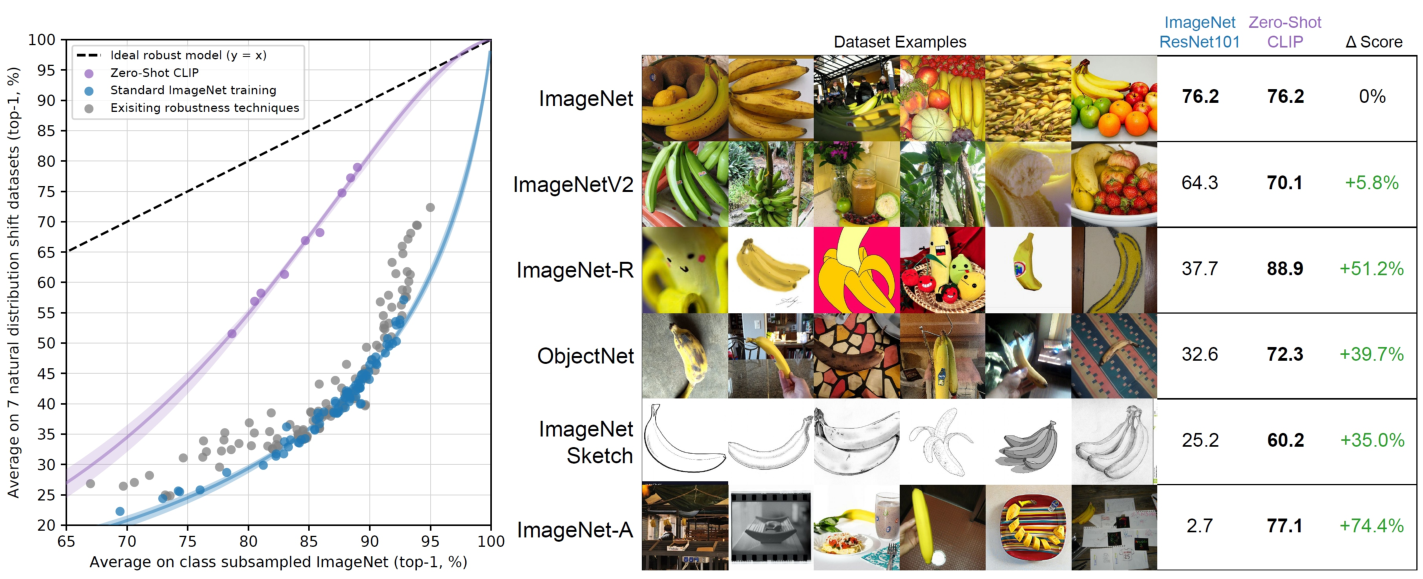
\includegraphics[width=0.85\textwidth]{../images/CLIP_Effective_Robustness_Dataset_Shift_mod.pdf}}

\footnote<.->{\tiny Radford, ICML, 2021}
\end{frame}

\begin{frame}{Large-scale Pre-Training and Transfer}
\protect\hypertarget{large-scale-pre-training-and-transfer-12}{}
\begin{itemize}
\tightlist
\item
  CLIP - language-vision foundation model; self-supervised
  language-vision learning (no labels)
\item
  Out-of-distribution robustness \& few-shot / zero-shot transfer
\item
  Pre-trained models are \textbf{highly re-usable across various tasks
  \& conditions}
\item
  Generalist zero-shot function: no adaptation to new conditions / data
  / tasks required
\end{itemize}

\center{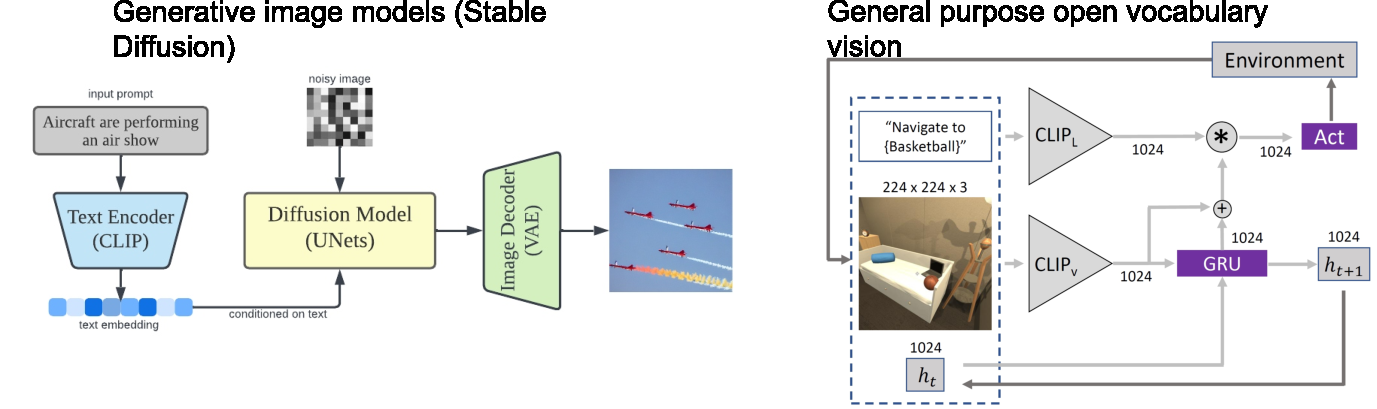
\includegraphics[width=0.9\textwidth]{../images/CLIP_re_usable_component_mod.pdf}}

\footnote<.->{\tiny Rombach et al, CVPR, 2022; Khandelwal et al, CVPR,
  2022}
\end{frame}

\begin{frame}{Large-scale Pre-Training and Transfer}
\protect\hypertarget{large-scale-pre-training-and-transfer-13}{}
\begin{itemize}
\tightlist
\item
  Problem - studying self-supervised foundation models is challenging:
  requires

  \begin{itemize}
  \tightlist
  \item
    large-scale \textbf{data} (at least 100M of samples)
  \item
    large-scale \textbf{compute} (in order of GPU months per single
    experiment)
  \item
    \textbf{expertise} in large-scale distributed training
  \end{itemize}
\end{itemize}

\center{
\includegraphics[width=0.2\textwidth]{../images/LAION_logo_mod.pdf}}

\begin{itemize}
\tightlist
\item
  Solution - LAION: Large-scale Artificial Intelligence Open Network

  \begin{itemize}
  \tightlist
  \item
    \textbf{data}: LAION-400M, LAION-5B image-text datasets --
    \textbf{Outstanding Paper Award NeurIPS 2022}
  \item
    \textbf{compute}: applying for publicly funded supercomputers
    (JUWELS, Germany, SUMMIT, USA)
  \item
    \textbf{expertise}: strong grassroot research community skilled in
    large-scale experiments and distributed training
  \item
    \textbf{Open-source} release of pre-trained models: openCLIP (work
    published at NeurIPS, CVPR)
  \end{itemize}
\end{itemize}
\end{frame}

\begin{frame}{Large-scale Pre-Training and Transfer}
\protect\hypertarget{large-scale-pre-training-and-transfer-14}{}
\begin{itemize}
\tightlist
\item
  LAION-400m/5B (2021): next gen datasets, 10x/100x larger than
  ImageNet-1k/21k, multi-modal (image-text)

  \begin{itemize}
  \tightlist
  \item
    data collection from public Internet (Common Crawl) by community
    effort (http://laion.ai)
  \end{itemize}
\item
  CommonPool-10B, DataComp-1B: follow-up work; systematic dataset search
  for pre-training strong models
\end{itemize}

\center{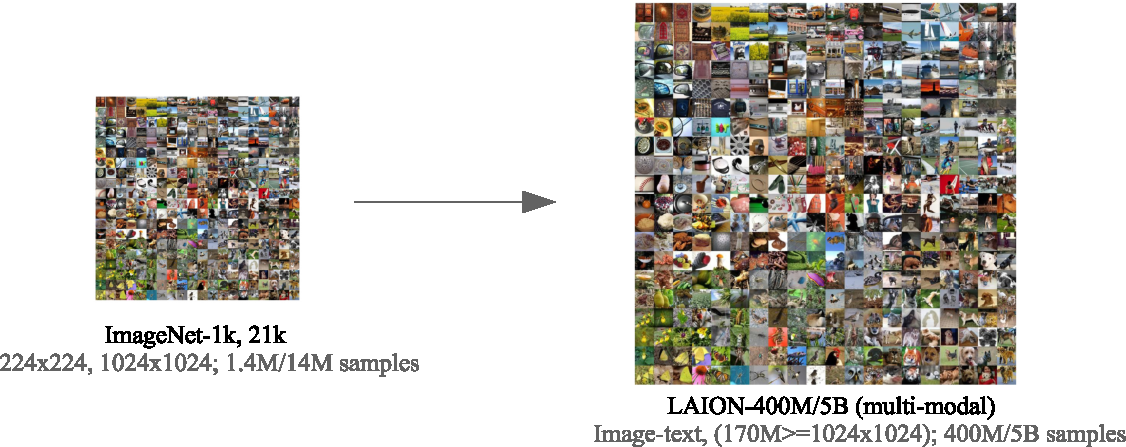
\includegraphics[width=0.8\textwidth]{../images/ImageNet_LAION_Transition_mod.pdf}}

\footnote<.->{\tiny  Schumann et al, NeurIPS 2022; Gadre, Ilharco, Fang
  et al, arXiv:2304.14108, 2023}
\end{frame}

\begin{frame}{Large-scale Pre-Training and Transfer}
\protect\hypertarget{large-scale-pre-training-and-transfer-15}{}
\begin{itemize}
\tightlist
\item
  Open data LAION-400M/5B, DataComp: Open sourcing data collection
  procedures

  \begin{itemize}
  \tightlist
  \item
    transparent dataset, open source tools \& workflows, reproducible
    training across various scales
  \item
    dataset of links to images in public internet, together with text
    captions
  \item
    researchers can obtain full image-text dataset for experiments using
    open tools
  \end{itemize}
\end{itemize}

\center{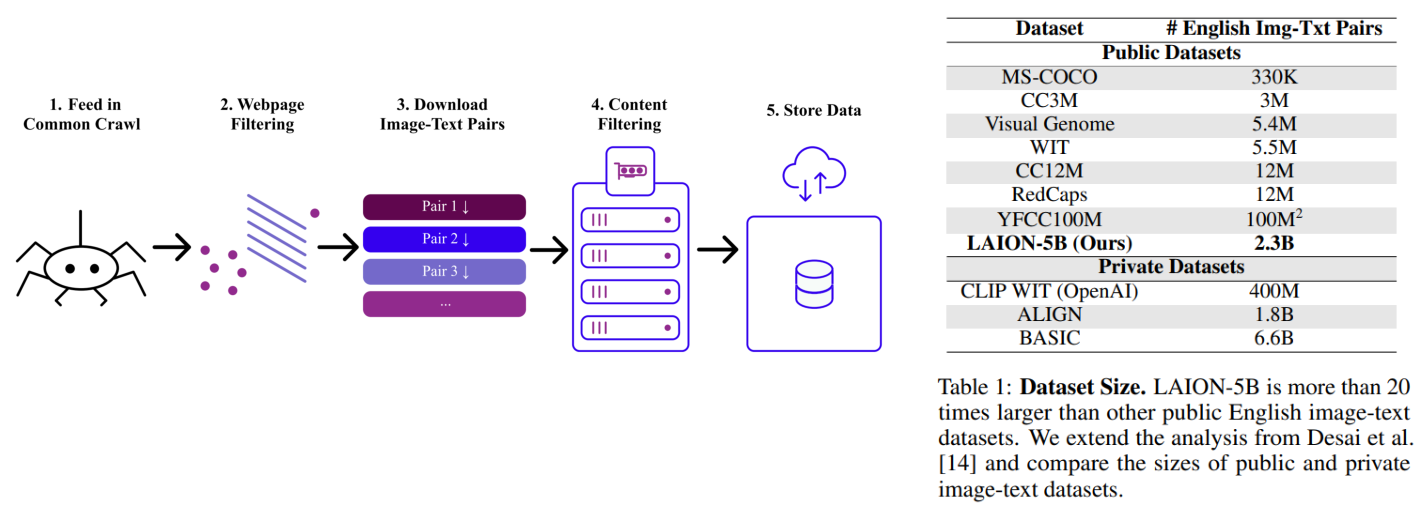
\includegraphics[width=0.9\textwidth]{../images/LAION_Dataset_mod.pdf}}

\footnote<.->{\tiny  Schumann et al, NeurIPS 2022; Gadre, Ilharco, Fang
  et al, arXiv:2304.14108, 2023}
\end{frame}

\begin{frame}{Large-scale Pre-Training and Transfer}
\protect\hypertarget{large-scale-pre-training-and-transfer-16}{}
\begin{itemize}
\tightlist
\item
  Open-source foundation data and models - reproducible, open science
\end{itemize}

\center{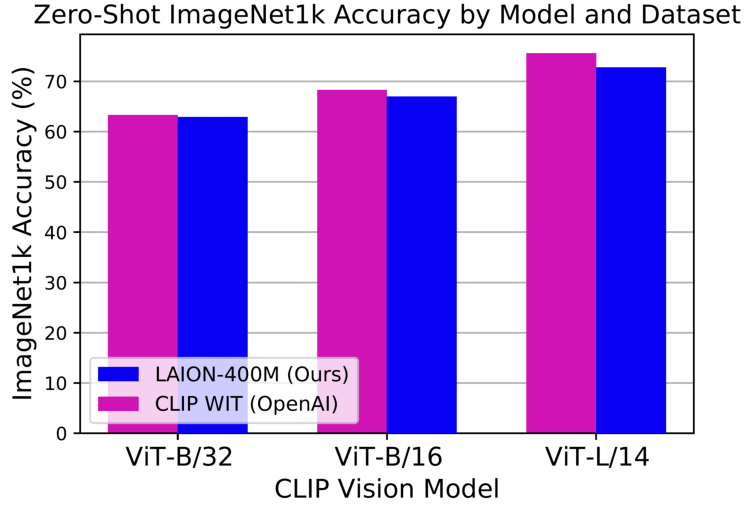
\includegraphics[width=0.7\textwidth]{../images/openCLIP_reproducible_LAION_comparison_plot_openAI_mod.pdf}}

\footnote<.->{\tiny  Schumann et al, NeurIPS 2022}
\end{frame}

\begin{frame}{Large-scale Pre-Training and Transfer}
\protect\hypertarget{large-scale-pre-training-and-transfer-17}{}
\begin{itemize}
\tightlist
\item
  Scaling laws for language-vision learning with LAION and openCLIP:
  open-source data, models and code - reproducible science
\end{itemize}

\center{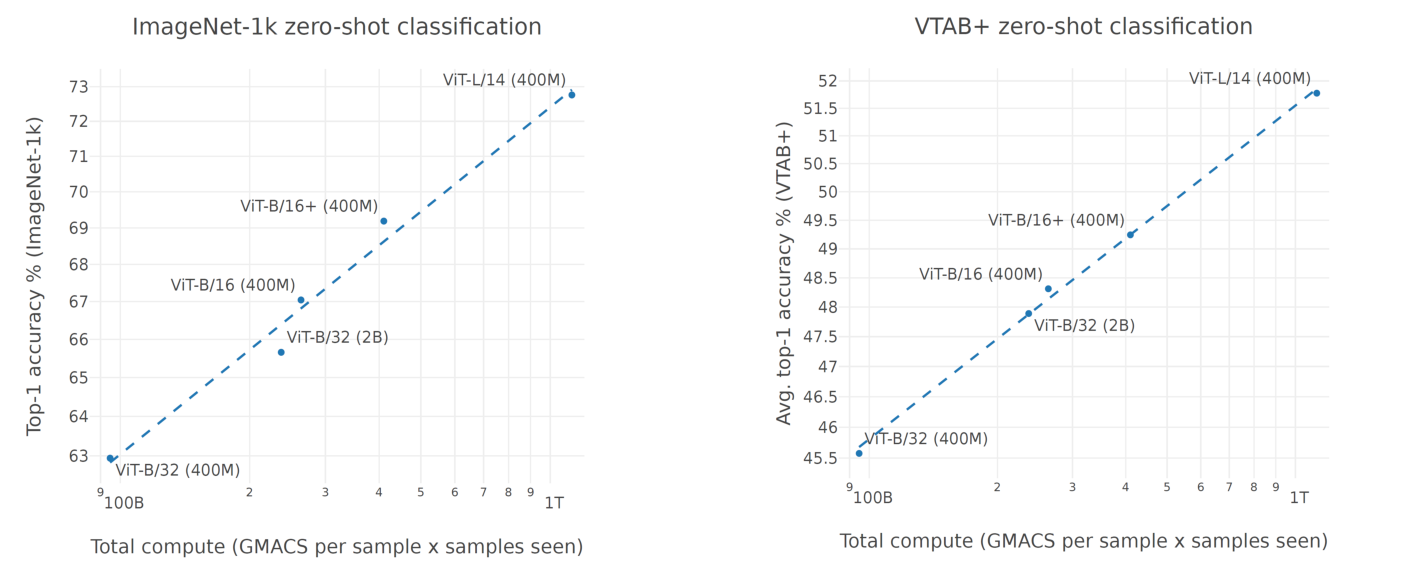
\includegraphics[width=\textwidth]{../images/LAION_openCLIP_scaling_zero_shot_mod.pdf}}

\footnote<.->{\tiny  Schumann et al, NeurIPS 2022}
\end{frame}

\begin{frame}{Large-scale Pre-Training and Transfer}
\protect\hypertarget{large-scale-pre-training-and-transfer-18}{}
\begin{itemize}
\tightlist
\item
  Scaling laws for language-vision learning with LAION and openCLIP:
  open-source data, models and code - reproducible science
\end{itemize}

\center{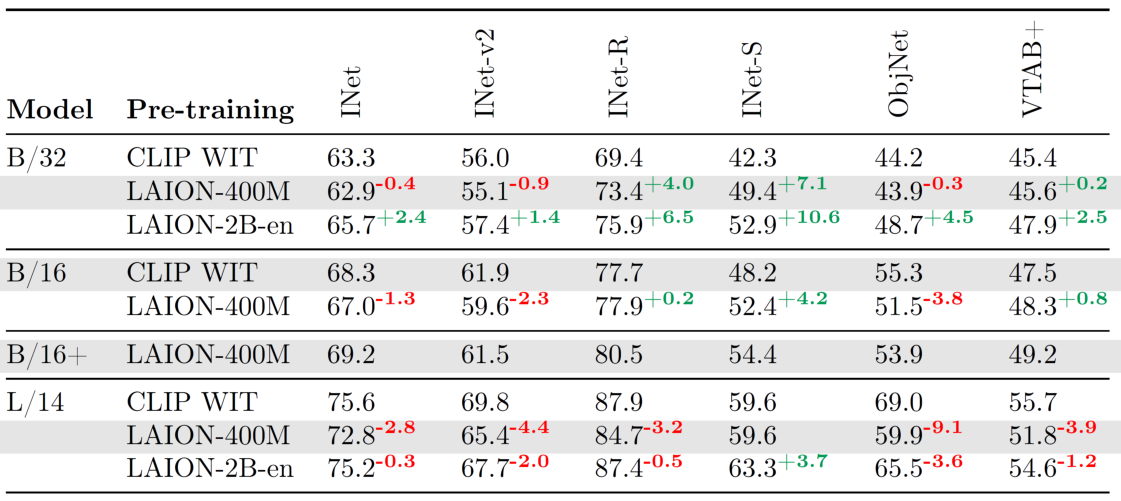
\includegraphics[width=0.9\textwidth]{../images/openCLIP_reproducible_LAION_table_mod.pdf}}

\footnote<.->{\tiny  Schumann et al, NeurIPS 2022}
\end{frame}

\begin{frame}{Large-scale Pre-Training and Transfer}
\protect\hypertarget{large-scale-pre-training-and-transfer-19}{}
\begin{itemize}
\tightlist
\item
  Bottlenecks: one insufficient scale can lead to saturation if
  increasing others
\item
  Larger language-vision models: stronger on larger dataset and sample
  seen scales
\end{itemize}

\center{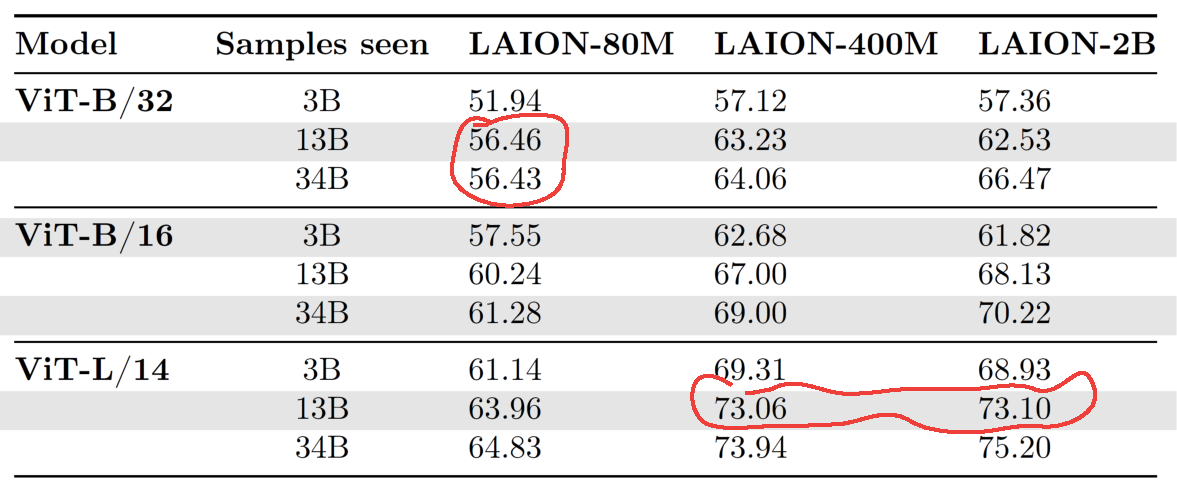
\includegraphics[width=0.9\textwidth]{../images/openCLIP_reproducible_LAION_scales_bottleneck_table_mod.pdf}}

\footnote<.->{\tiny Cherti et al, arXiv:2212.07143, CVPR 2023}
\end{frame}

\begin{frame}{Large-scale Pre-Training and Transfer}
\protect\hypertarget{large-scale-pre-training-and-transfer-20}{}
\begin{itemize}
\tightlist
\item
  Scaling laws for language-vision learning with LAION and openCLIP:
  open-source data, models and code - reproducible science
\item
  Predicting model performance and properties on larger scales
\end{itemize}

\center{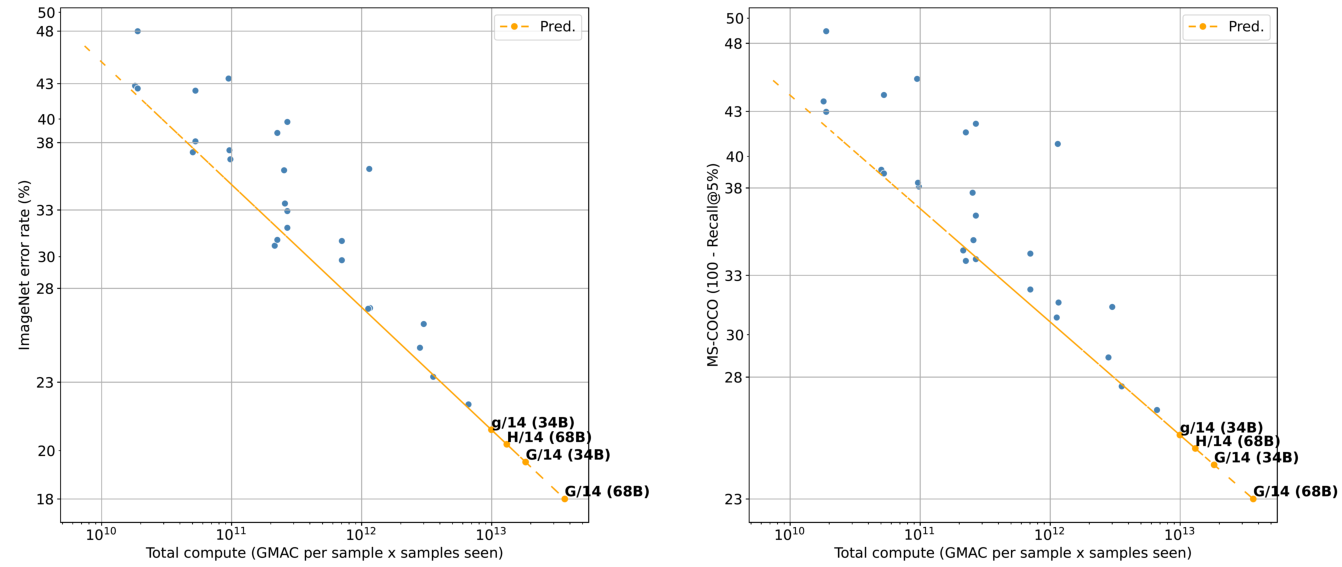
\includegraphics[width=\textwidth]{../images/openCLIP_reproducible_LAION_scaling_law_prediction_mod.pdf}}

\footnote<.->{\tiny Cherti et al, arXiv:2212.07143, CVPR 2023}
\end{frame}

\begin{frame}{Large-scale Pre-Training and Transfer}
\protect\hypertarget{large-scale-pre-training-and-transfer-21}{}
\begin{itemize}
\tightlist
\item
  Scaling laws for language-vision learning with LAION and openCLIP:
  open-source data, models and code - reproducible science
\item
  Predicting model performance and properties on larger scales
\end{itemize}

\center{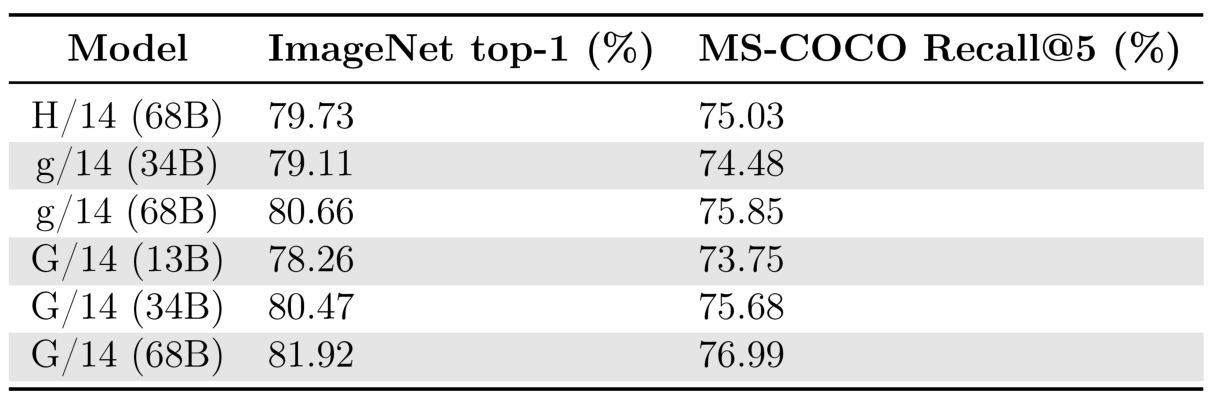
\includegraphics[width=0.9\textwidth]{../images/openCLIP_reproducible_LAION_scaling_law_prediction_table_mod.pdf}}

\footnote<.->{\tiny Cherti et al, arXiv:2212.07143, CVPR 2023}
\end{frame}

\begin{frame}{Large-scale Pre-Training and Transfer}
\protect\hypertarget{large-scale-pre-training-and-transfer-22}{}
\begin{itemize}
\tightlist
\item
  JUWELS Booster: necessary for the experiments
\item
  122 hours with 1024 A100 (124K GPU hours) for training of ViT L/14
  openCLIP on 34B samples
\item
  In contrast to standard supervised training: larger batch sizes
  beneficial for learning
\end{itemize}

\center{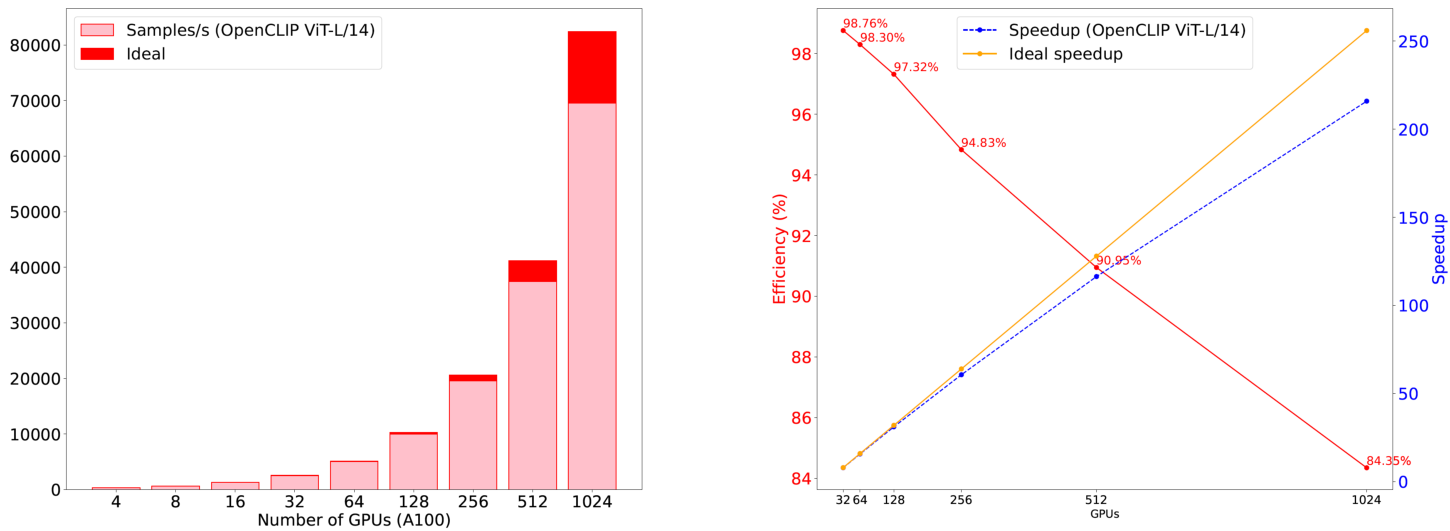
\includegraphics[width=\textwidth]{../images/openCLIP_scaling_efficiency_plots_L14_mod.pdf}}

\footnote<.->{\tiny Cherti et al, arXiv:2212.07143, CVPR 2023}
\end{frame}

\begin{frame}{Large-scale Pre-Training and Transfer}
\protect\hypertarget{large-scale-pre-training-and-transfer-23}{}
\begin{itemize}
\tightlist
\item
  Current language-vision models are still small scale (compared to LLMs
  (\textgreater100B params); PaLI (image-text-to-text) -- 17B; Parti
  (text-to-image) - 20B params)
\item
  Stronger transfer \& robustness: aiming for larger scales
\item
  Larger machines necessary: JUPITER Exascale upcoming at JSC
\end{itemize}

\center{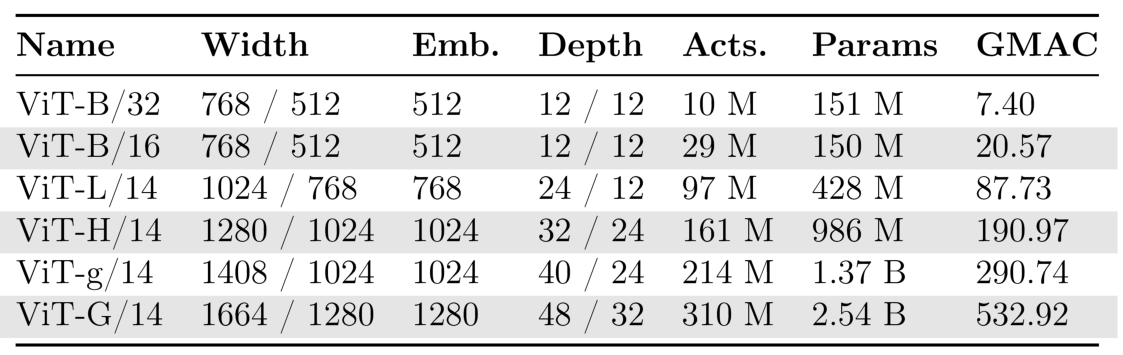
\includegraphics[width=0.9\textwidth]{../images/openCLIP_GMAC_params_table_mod.pdf}}

\footnote<.->{\tiny Cherti et al, arXiv:2212.07143, CVPR 2023}
\end{frame}

\begin{frame}{Distributed Training with Very Large Models}
\protect\hypertarget{distributed-training-with-very-large-models}{}
\begin{itemize}
\tightlist
\item
  Growing model scale: only data parallel scheme not sufficient

  \begin{itemize}
  \tightlist
  \item
    Language Modelling: GPT-3 - 175 Billion parameters; PaLM (Google) -
    540B parameters
  \item
    Vision: ViT-22B; Language-Vision: Parti - 17B params
  \end{itemize}
\item
  Model/Tensor parallelism, Pipeline Parallelism: can split a very large
  model across accelerators
\item
  Different libraries: DeepSpeed (Microsoft), CollosalAI (HPC-AI),
  PyTorch/TensorFlow DTensor, \ldots{}
\end{itemize}

\center{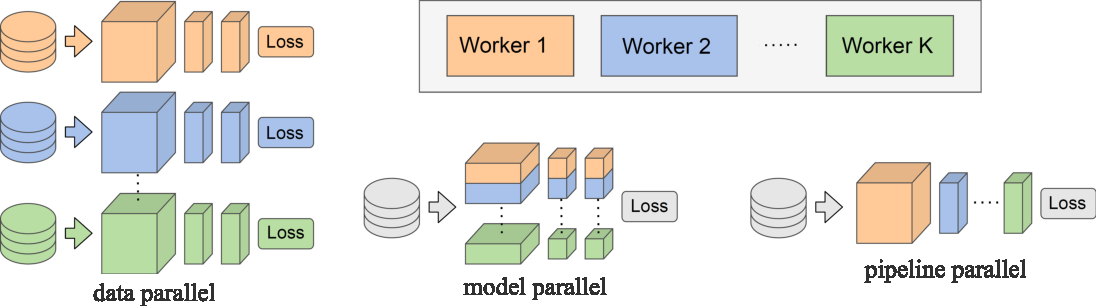
\includegraphics[width=\textwidth]{../images/Distributed_Training_Schemes_Titled_Slides.pdf}}

\footnote<.->{\tiny Laskin et al, 2020}
\end{frame}

\begin{frame}{Distributed Training with Very Large Models}
\protect\hypertarget{distributed-training-with-very-large-models-1}{}
\begin{itemize}
\tightlist
\item
  Hybrid parallel schemes

  \begin{itemize}
  \tightlist
  \item
    using data, model and pipeline parallelism simultaneously
  \end{itemize}
\item
  Distributed training that combines memory and compute efficiency
\item
  DeepSpeed: supports hybrid parallelism
\end{itemize}

\center{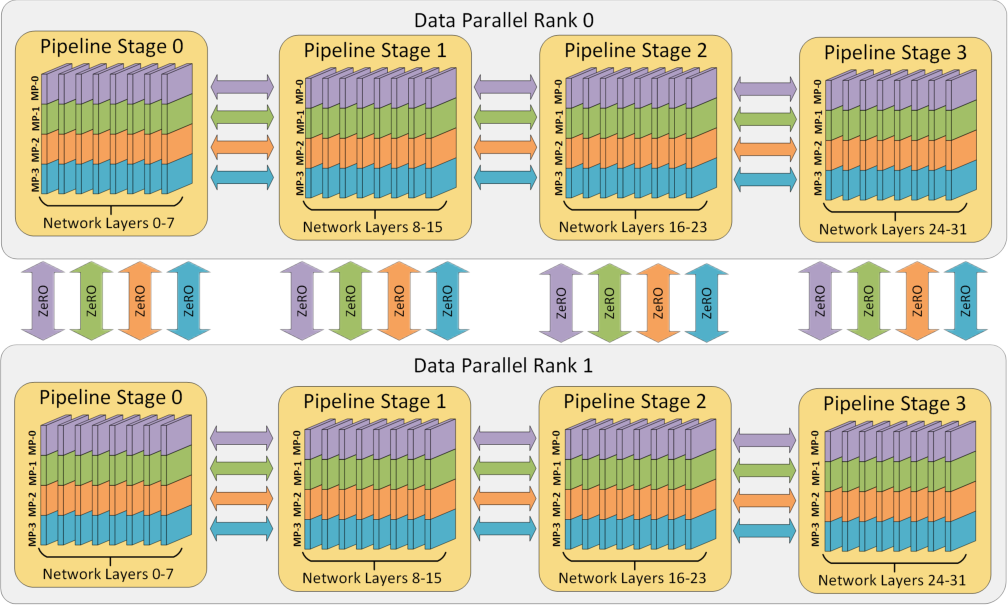
\includegraphics[width=0.7\textwidth]{../images/DeepSpeed_Hybrid_Parallel_Slide.pdf}}
\end{frame}

\begin{frame}{Distributed Training with Very Large Models}
\protect\hypertarget{distributed-training-with-very-large-models-2}{}
\begin{itemize}
\tightlist
\item
  Hybrid parallel schemes

  \begin{itemize}
  \tightlist
  \item
    using data, model and pipeline parallelism simultaneously
  \end{itemize}
\item
  DeepSpeed: ``3D Parallelism''

  \begin{itemize}
  \tightlist
  \item
    executing and speeding up a Trillion size model on 800 A100 GPUs
  \end{itemize}
\end{itemize}

\center{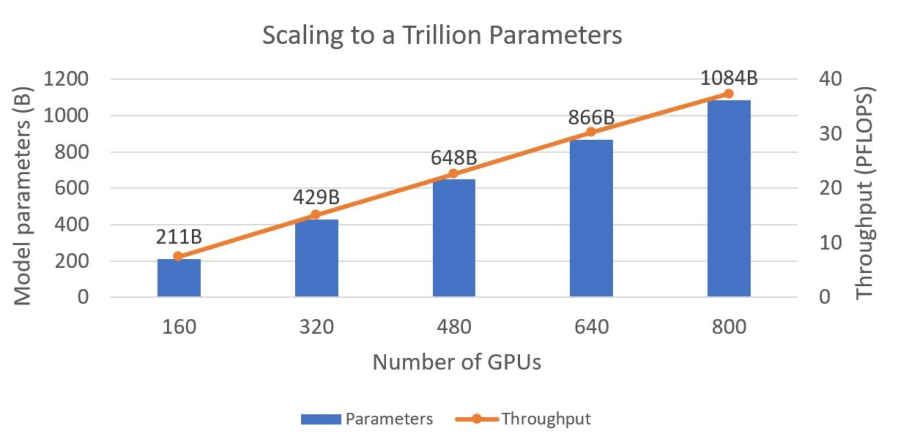
\includegraphics[width=0.8\textwidth]{../images/DeepSpeed_Scaling_Slide.pdf}}
\end{frame}

\begin{frame}{Distributed Training with Very Large Models}
\protect\hypertarget{distributed-training-with-very-large-models-3}{}
\begin{itemize}
\tightlist
\item
  Upcoming: local updates, decoupled gradients
\item
  Getting rid of global forward-backward pass dependency alltogether
\item
  Asynchronous local updates, highly beneficial for parallelization
\item
  Towards energy-efficient in-memory computing: minimize data transfer
\item
  New generic losses for unsupervised learning
\end{itemize}

\center{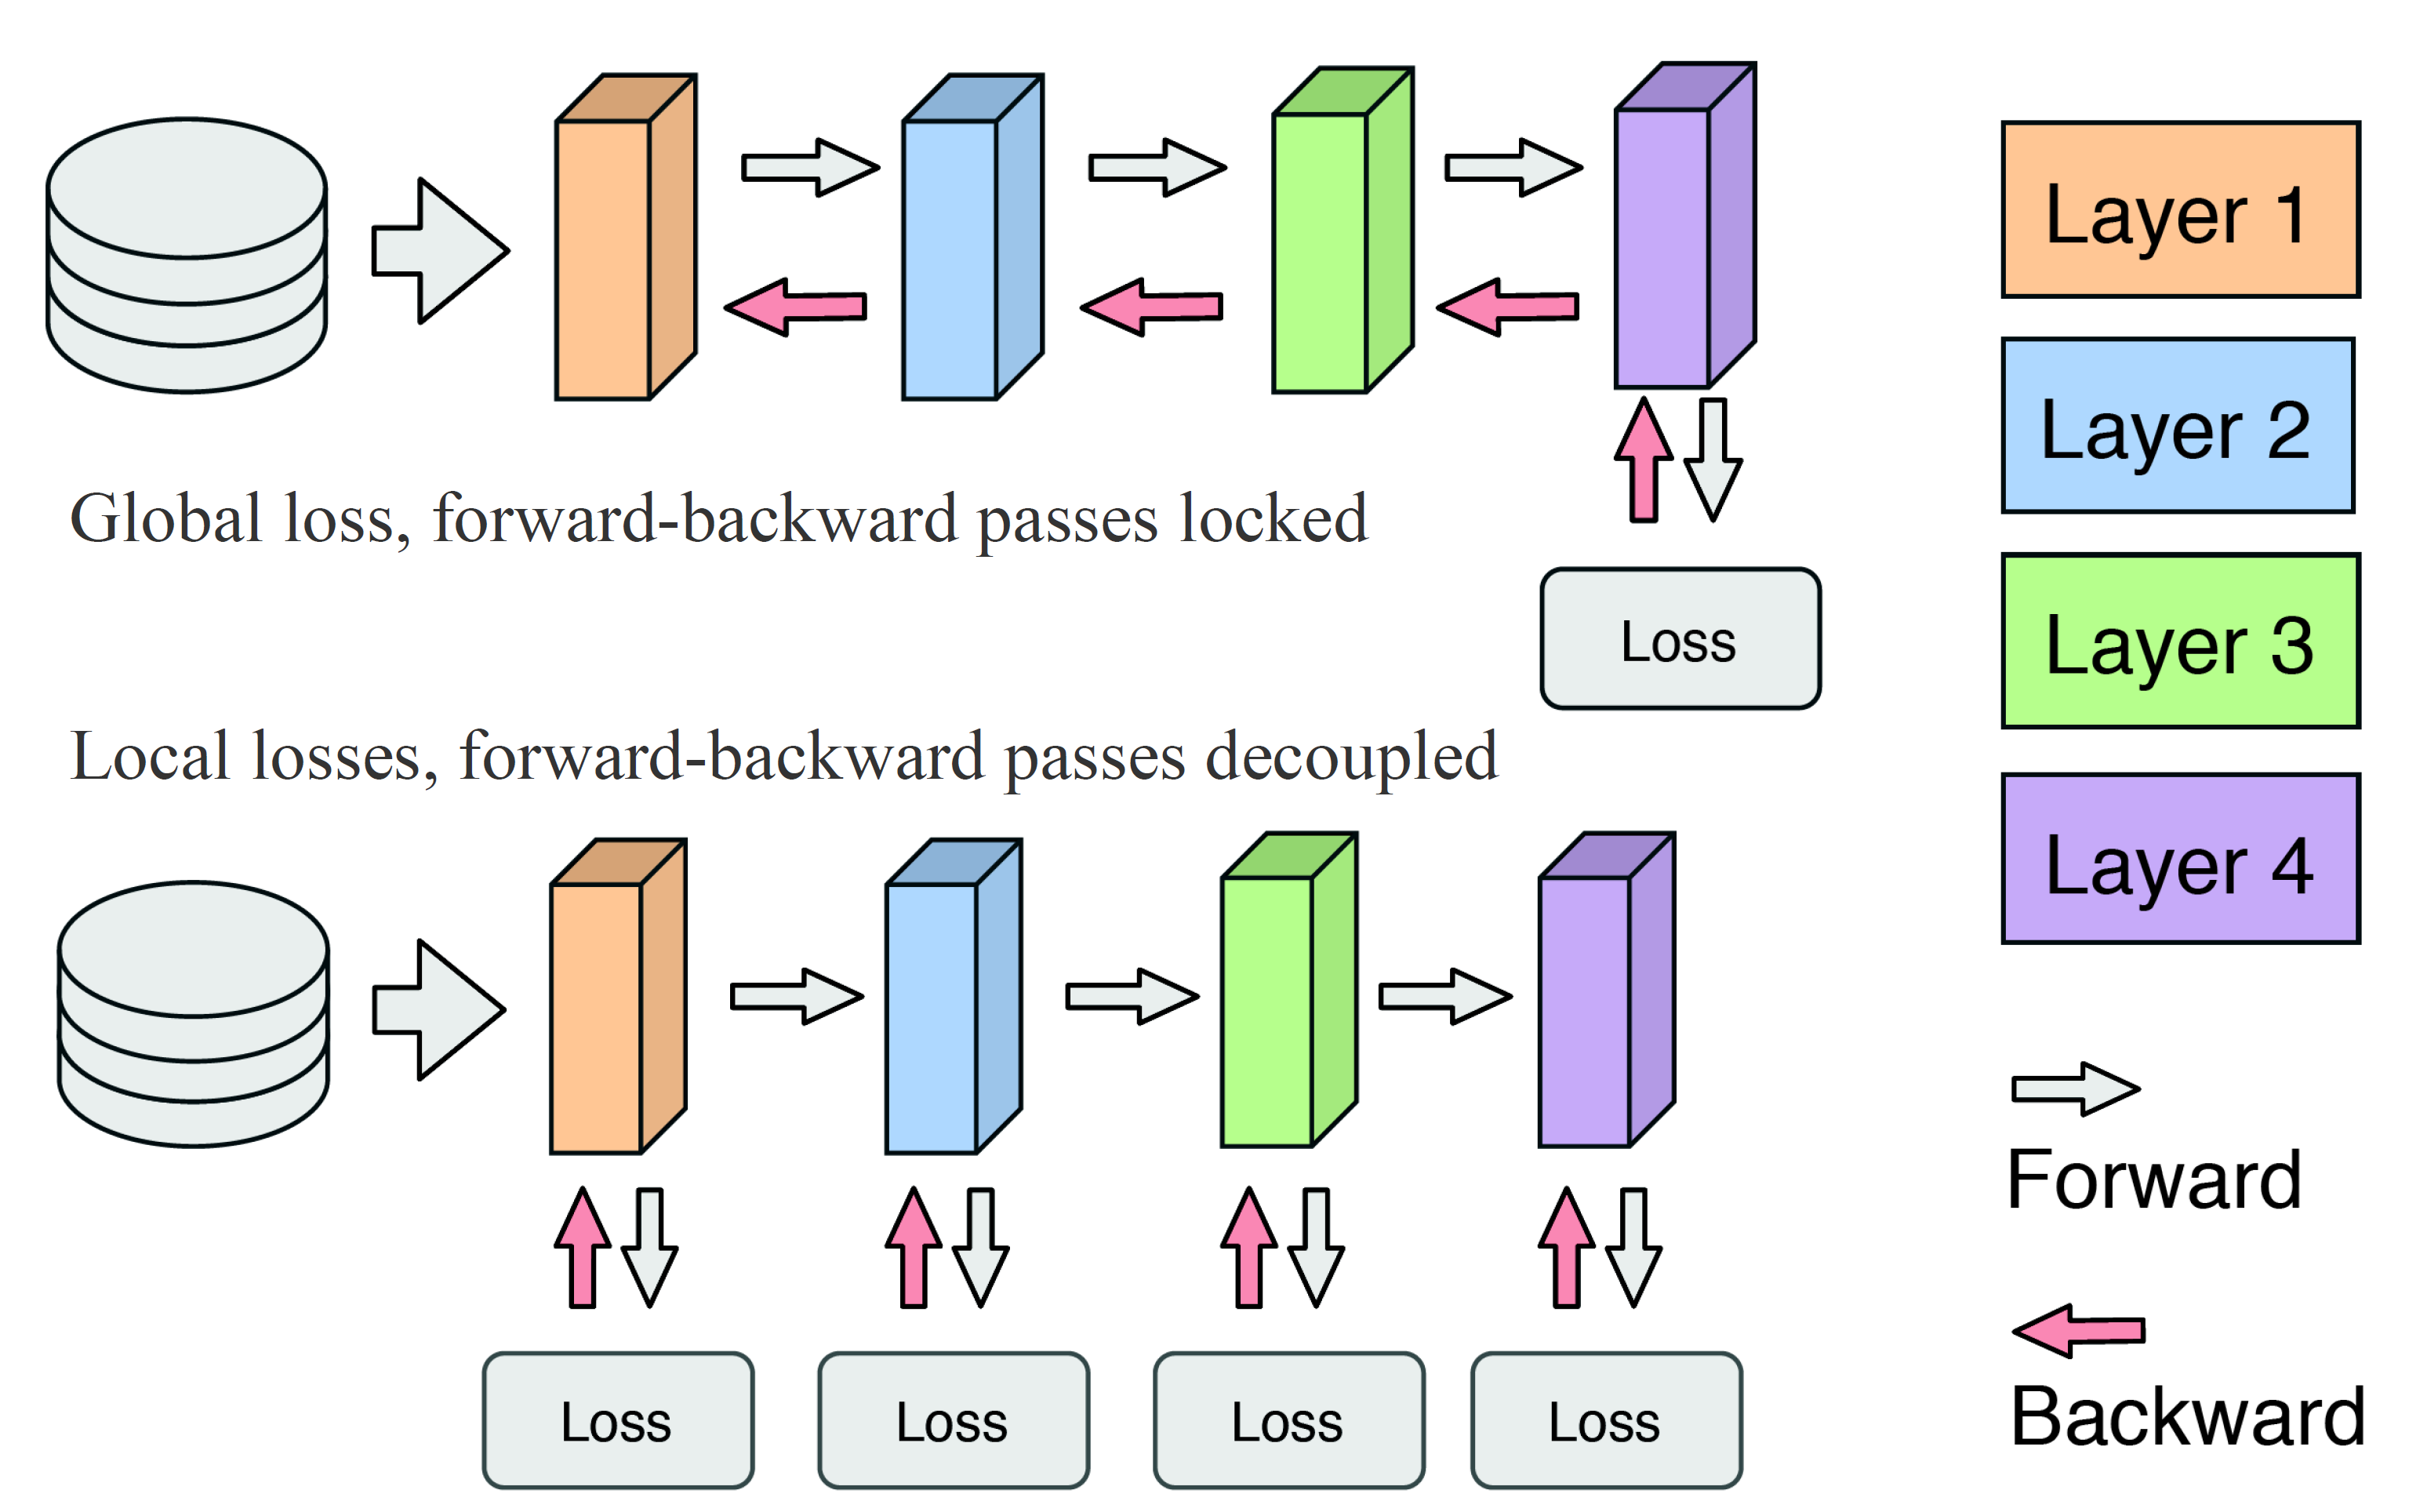
\includegraphics[width=0.5\textwidth]{../images/Local_Losses_Decoupled_Slide.png}}

\footnote<.->{\tiny Laskin et al, 2020}
\end{frame}

\begin{frame}{Distributed Training with Very Large Models}
\protect\hypertarget{distributed-training-with-very-large-models-4}{}
\begin{itemize}
\tightlist
\item
  Upcoming: local updates, decoupled gradients
\item
  Asynchronous local updates, highly beneficial for parallelization
\item
  Energy efficient distributed training on specialized hardware,
  in-memory computing

  \begin{itemize}
  \tightlist
  \item
    Graphcore IPU: Colossus Mk2
  \item
    Cerebras : Wafer Scale Engine 2 (WSE - 850k Cores!)
  \end{itemize}
\end{itemize}

\center{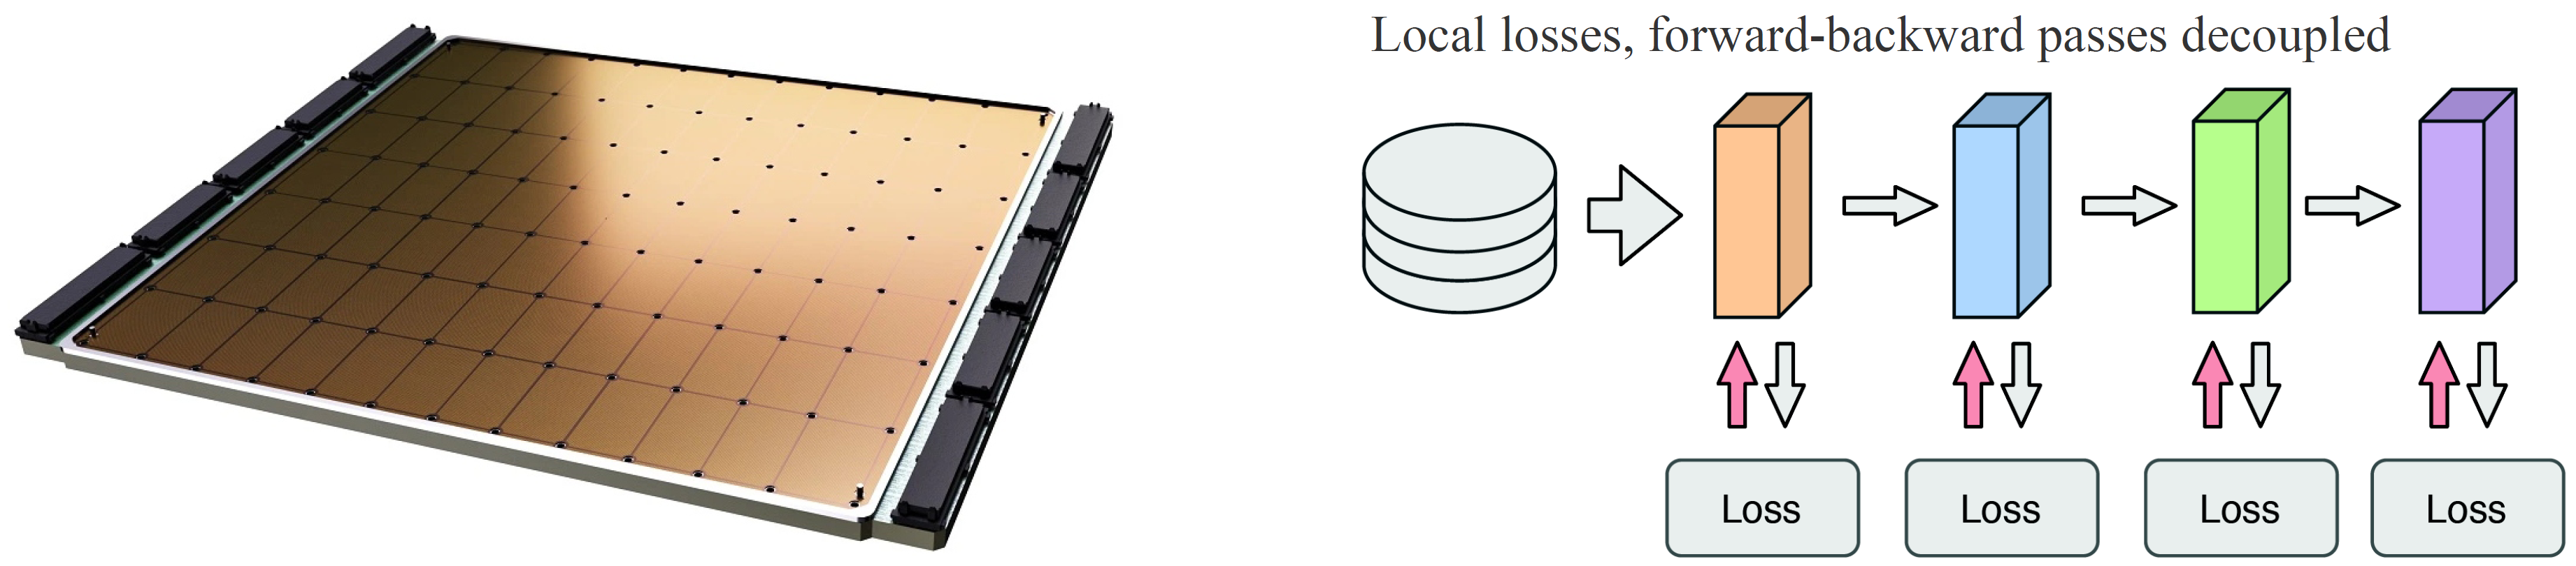
\includegraphics[width=\textwidth]{../images/Cerebras_Local_Losses_Slide.png}}
\end{frame}

\begin{frame}{Large-Scale Foundation Generalist Models}
\protect\hypertarget{large-scale-foundation-generalist-models}{}
\begin{block}{Outlook}
\protect\hypertarget{outlook}{}
\begin{itemize}
\tightlist
\item
  Language-vision generalist models for strong transfer across domains
  and tasks
\item
  Large model scale: hybrid parallelism required
\item
  Large data scale: data collection and automated filtering (see
  DataComp)
\item
  Systematic Search for Scalable Architectures (Project Nucleus, LAION)
\item
  Model compression for efficient transfer and low resource deployment
\item
  Energy efficient large scale learning with in-memory computing
  neuromorphic hardware
\end{itemize}
\end{block}

\center{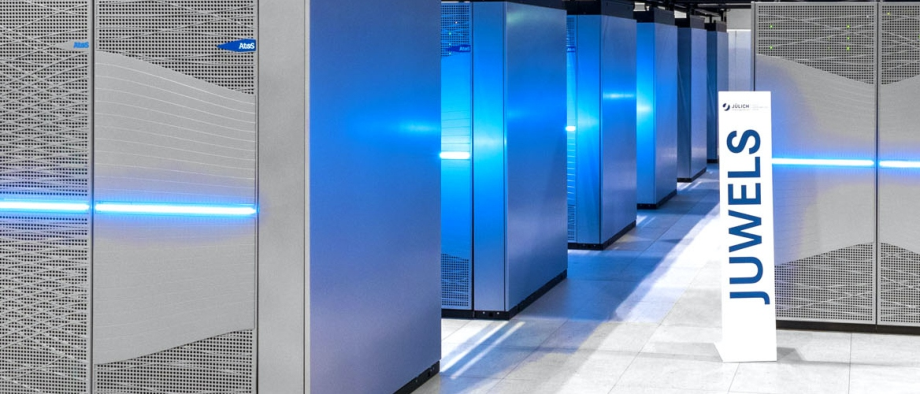
\includegraphics[width=0.6\textwidth]{../images/JUWELS_Booster_Slide.pdf}}
\end{frame}

\begin{frame}{Large-Scale Foundation Generalist Models}
\protect\hypertarget{large-scale-foundation-generalist-models-1}{}
\begin{itemize}
\tightlist
\item
  LAION: Large-Scale Artificial Intelligence Open Network (join on
  Discord!)

  \begin{itemize}
  \tightlist
  \item
    Scalable Learning \& Multi-Purpose Lab (SLAMPAI; Jenia Jitsev, Mehdi
    Cherti)
  \item
    University of Washington (Seattle), Allen AI Institute, MILA, UC
    Berkeley, U Tel-Aviv, Stanford, \ldots{}
  \item
    https://laion.ai/ - join on Discord!
  \end{itemize}
\item
  Supercomputers : JUWELS \& JUWELS Booster, JUPITER to come
\end{itemize}

\center{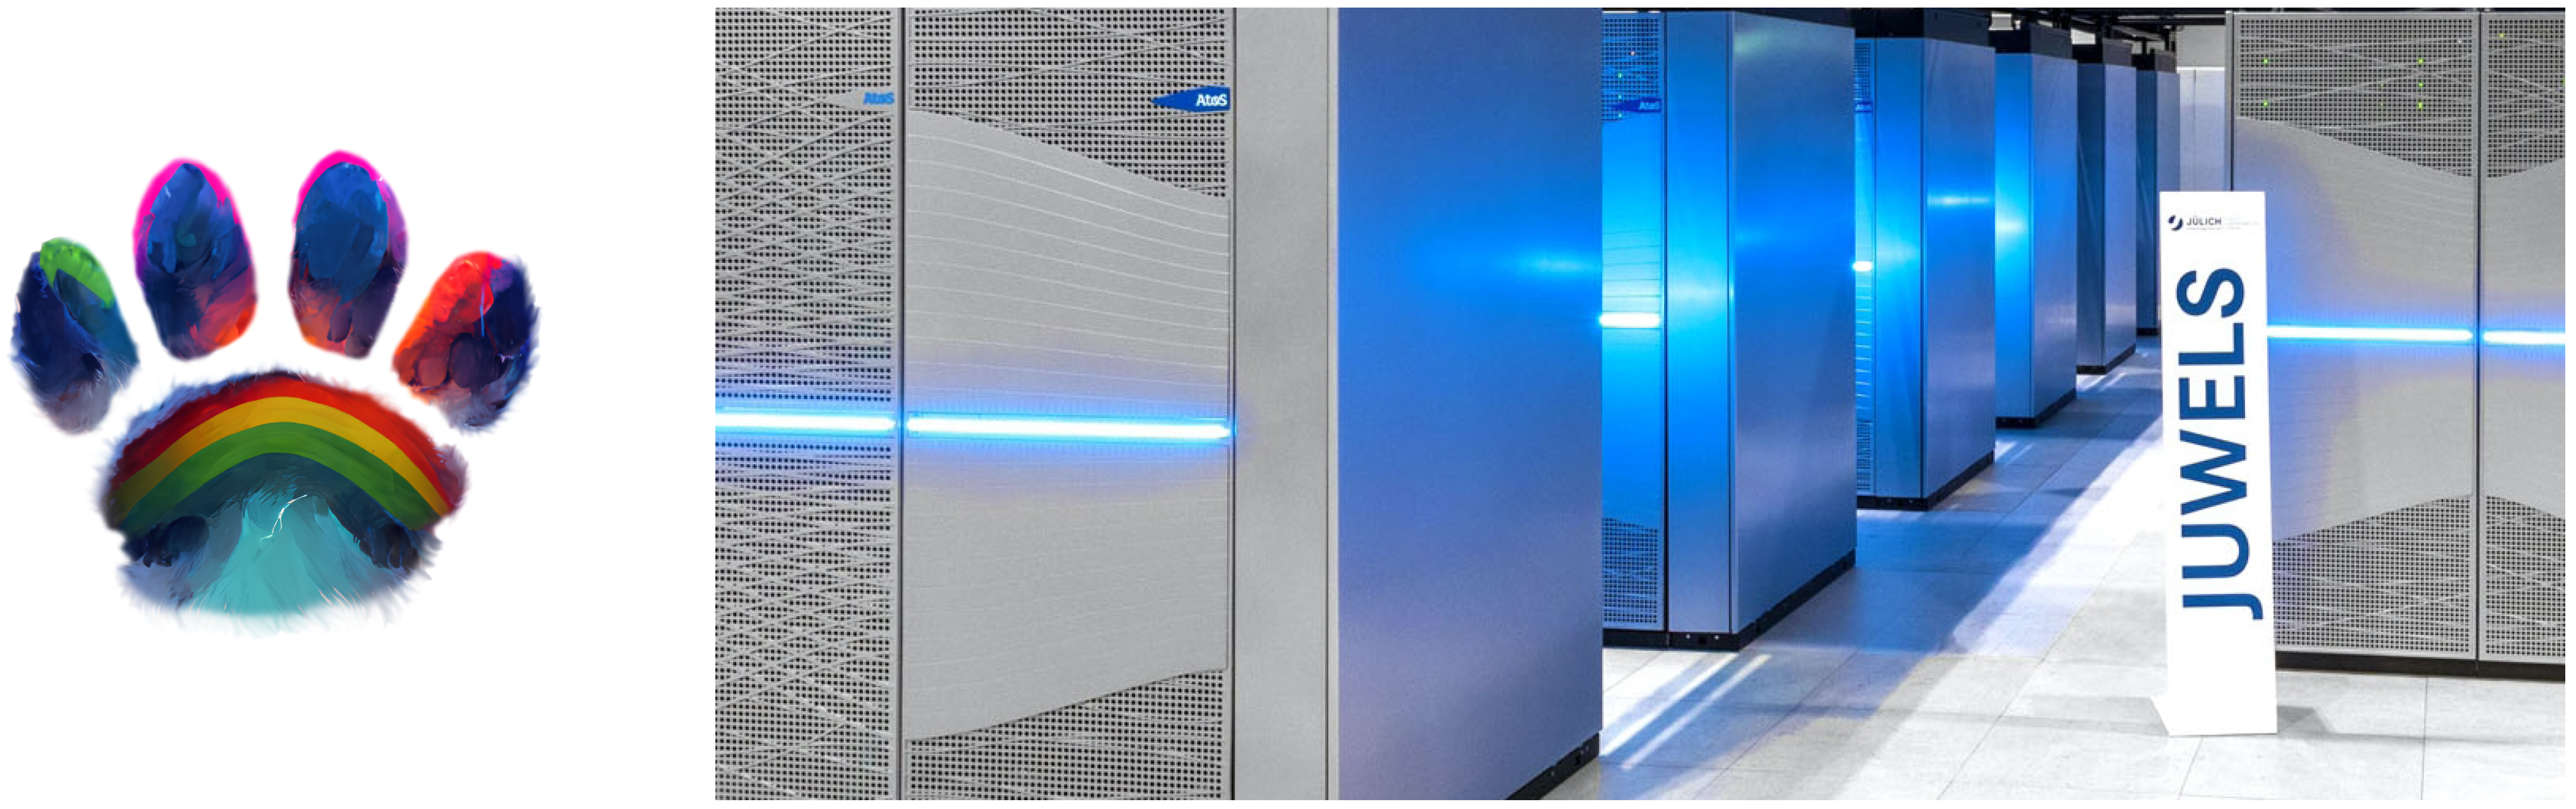
\includegraphics[width=0.8\textwidth]{../images/LAION_JUWELS.png}}
\end{frame}

\begin{frame}{Large-Scale Foundation Generalist Models}
\protect\hypertarget{large-scale-foundation-generalist-models-2}{}
\begin{itemize}
\tightlist
\item
  WestAI: AI Service Center, funded by BMBF (2022-2025, 12.4M €)
\item
  Pillars: large-scale pre-training, scaling laws for transfer,
  compression, next-gen highly scalable generic, energy-efficient
  learning

  \begin{itemize}
  \tightlist
  \item
    SLAMPAI at JSC: scientific lead
  \item
    U Bonn, RWTH Aachen, Fraunhofer IAIS, U Padeborn, U Dortmund
  \end{itemize}
\end{itemize}

\center{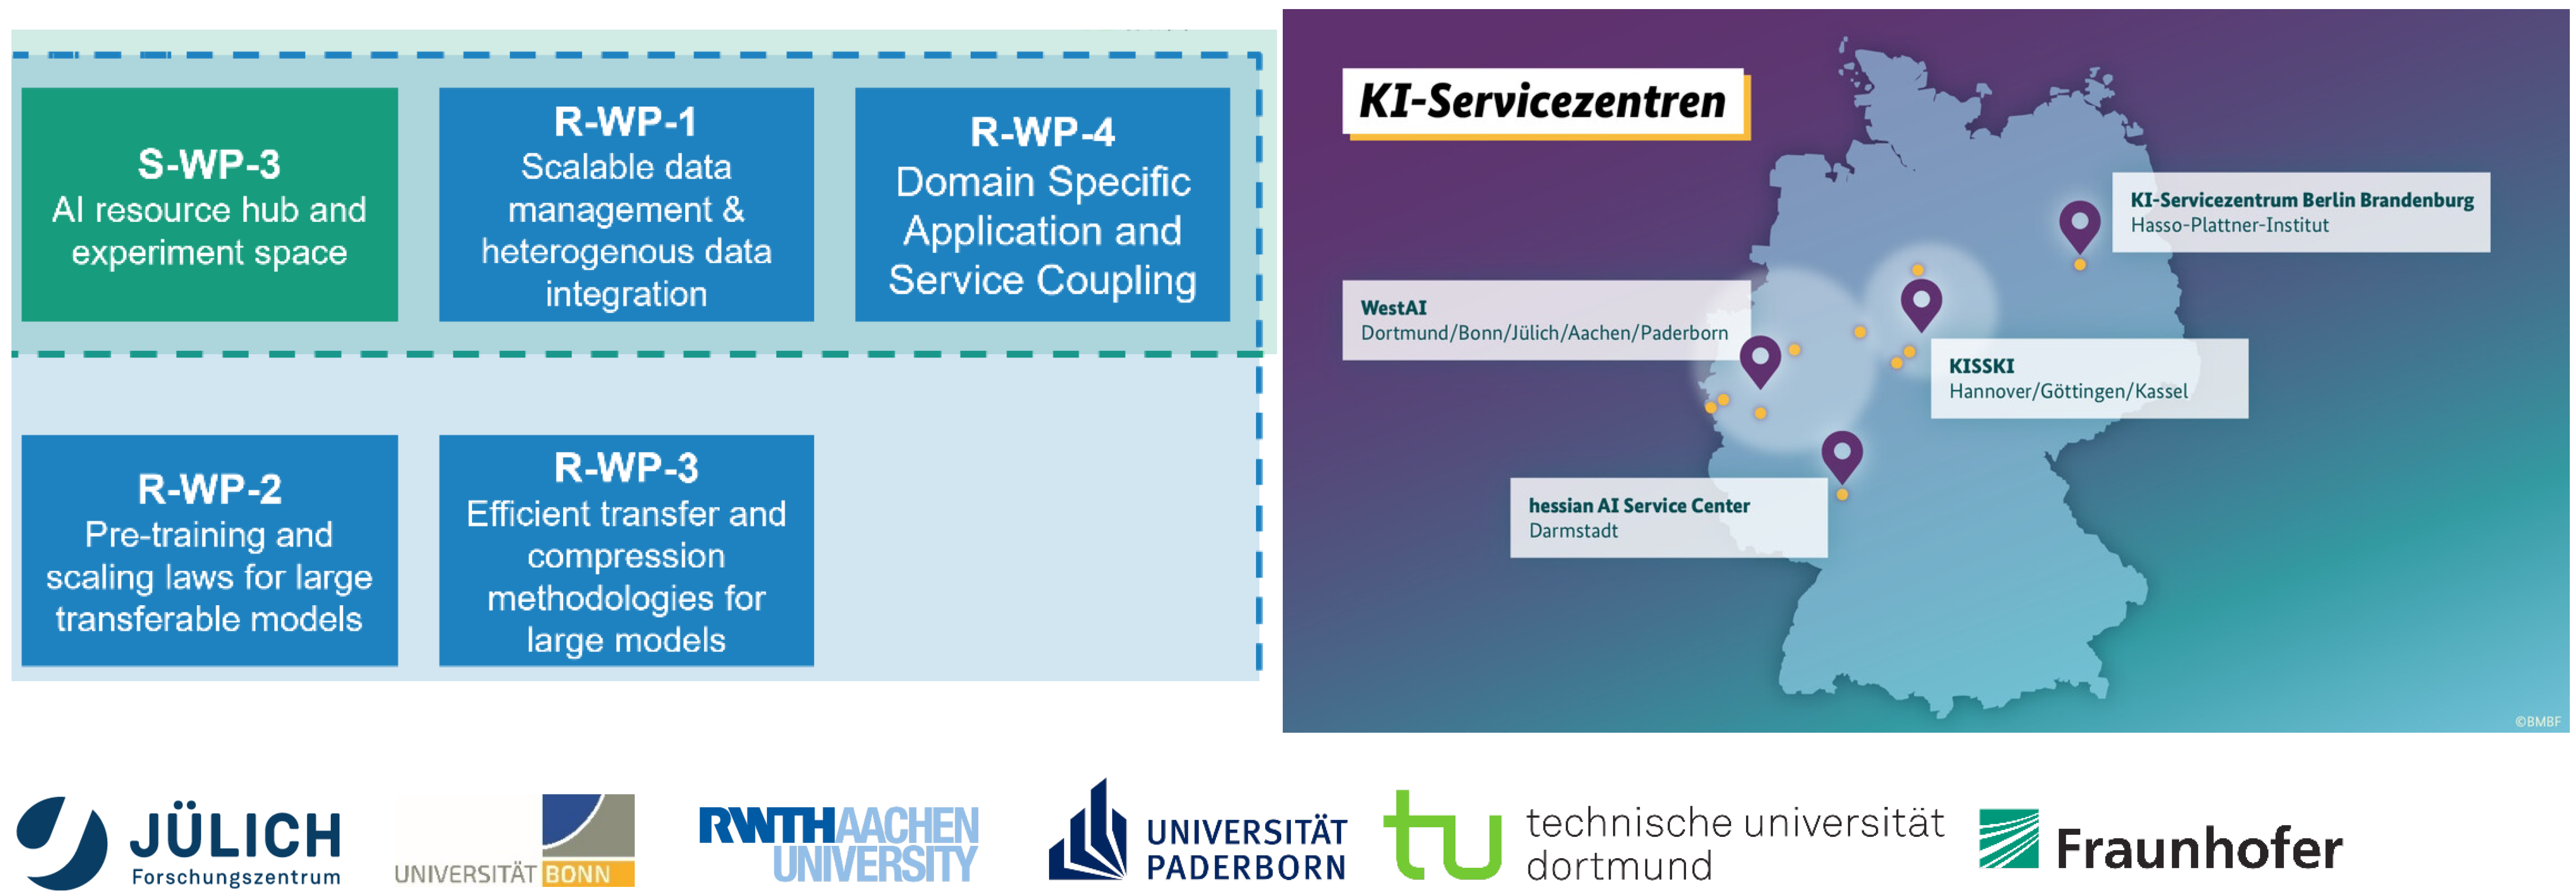
\includegraphics[width=0.9\textwidth]{../images/WestAI_Consortium.png}}
\end{frame}

\begin{frame}{Distributed Training: Activities at FZJ}
\protect\hypertarget{distributed-training-activities-at-fzj}{}
\begin{itemize}
\tightlist
\item
  Distributed Training for Hyperspectral Remote Sensing (Gabriele
  Cavallaro)
\item
  Helmholtz Data Challenges : Platform for collaborative datasets and
  model training

  \begin{itemize}
  \tightlist
  \item
    SLAMPAI \& Helmholtz AI Consultant Team:
    https://helmholtz-data-challenges.de/
  \end{itemize}
\item
  TOAR: Earth System Data Exploration (ESDE) Lab (Martin Schultz)
\item
  Helmholtz AI Research Group at INM-1: deep learning for neuroimaging
\item
  JULAIN: Juelich Artificial Intelligence Network, join in!

  \begin{itemize}
  \tightlist
  \item
    mailing list: https://lists.fz-juelich.de/mailman/listinfo/ml
  \end{itemize}
\end{itemize}

\center{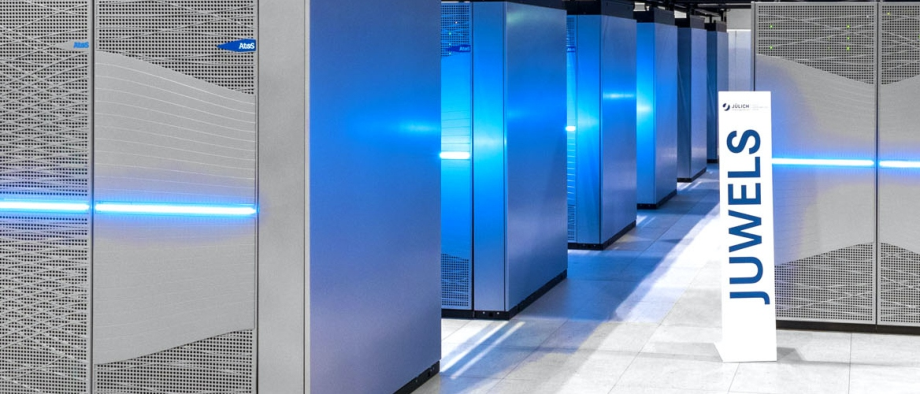
\includegraphics[width=0.6\textwidth]{../images/JUWELS_Booster_Slide.pdf}}
\end{frame}

\begin{frame}{Large-Scale Foundation Generalist Models}
\protect\hypertarget{large-scale-foundation-generalist-models-3}{}
\begin{itemize}
\tightlist
\item
  LAION: Large-Scale Artificial Intelligence Open Network (join on
  Discord!)

  \begin{itemize}
  \tightlist
  \item
    Scalable Learning \& Multi-Purpose Lab (SLAMPAI; Jenia Jitsev, Mehdi
    Cherti)
  \item
    University of Washington (Seattle), Allen AI Institute, MILA, UC
    Berkeley, U Tel-Aviv, Stanford, \ldots{}
  \item
    https://laion.ai/ - join on Discord!
  \end{itemize}
\item
  Supercomputers : JUWELS \& JUWELS Booster, JUPITER to come
\end{itemize}

\center{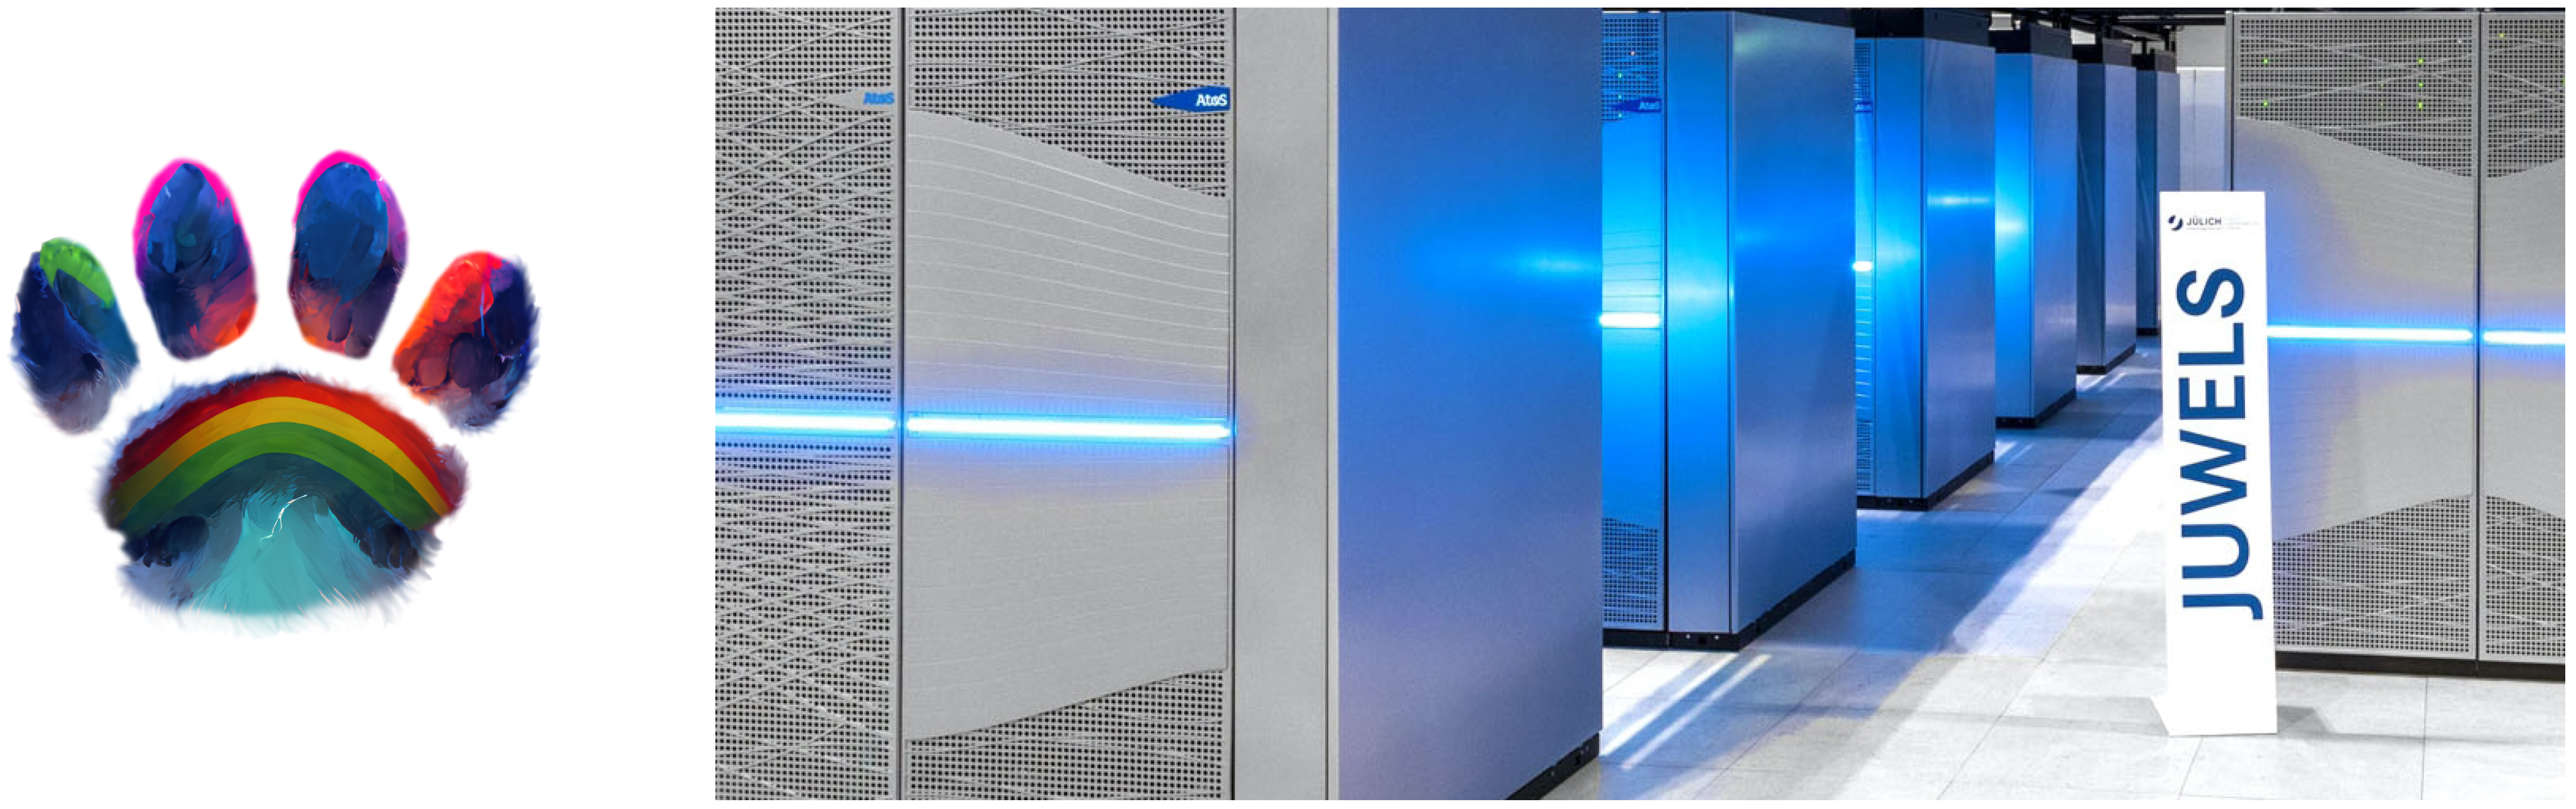
\includegraphics[width=0.8\textwidth]{../images/LAION_JUWELS.png}}
\end{frame}
